%% ============================================================
%% EXAMEN FINAL – ECONOMETRÍA INTERMEDIA: MACRO | 2026-1 | PUCP
%%
%% Autores : Andrea Quispe, Valeria Avilés
%%           Ventura Meza, Alejandro
%% Profesor: Erick Lahura
%% JP      : Juan Diego Goicochea
%% ============================================================

\documentclass[12pt, letterpaper]{article}

%% --- Tipografía: Times New Roman ---
\usepackage{mathptmx}
\usepackage[T1]{fontenc}
\usepackage[utf8]{inputenc}
\usepackage[spanish, es-tabla]{babel}

%% --- Márgenes (estándar universitario) ---
\usepackage[top=2.54cm, bottom=2.54cm,
            left=2.54cm,  right=2.54cm]{geometry}

%% --- Espaciado 1.15 ---
\usepackage{setspace}
\setstretch{1.15}

%% --- Fix: incompatibilidad setspace/booktabs ---
\usepackage{etoolbox}
\AtBeginEnvironment{tabular}{\setstretch{1}}
\AtBeginEnvironment{tablenotes}{\setstretch{1}}

%% --- Matemáticas ---
\usepackage{amsmath, amssymb}

%% --- Tablas ---
\usepackage{booktabs}
\usepackage{multirow}
\usepackage{array}
\usepackage{adjustbox}
\usepackage{threeparttable}
\usepackage{longtable}
\usepackage{caption}
\captionsetup{font=small, labelfont=bf, labelsep=period}

%% --- Figuras ---
\usepackage{graphicx}
\usepackage{subcaption}
\usepackage{float}
\graphicspath{{figures/}}

%% --- Código fuente (EViews, Python) ---
\usepackage{xcolor}
\usepackage{listings}
\lstdefinelanguage{EViews}{
  morekeywords={smpl,series,equation,group,graph,table,show,for,next,var,system,append,sur,ls,cointreg,uroot,coint,makeresid,freeze,scalar,param,append},
  sensitive=false,
  morecomment=[l]{'},
  morestring=[b]",
}
\lstset{
  basicstyle=\ttfamily\scriptsize,
  breaklines=true,
  frame=single,
  numbers=left,
  numberstyle=\tiny\color{gray},
  columns=fullflexible,
  keywordstyle=\color{blue!60!black}\bfseries,
  commentstyle=\color{green!40!black}\itshape,
  stringstyle=\color{orange!70!black},
  backgroundcolor=\color{gray!5},
  breakautoindent=false,
  breakindent=0pt,
  extendedchars=true,
  inputencoding=utf8,
  literate=
    {á}{{\'a}}1 {é}{{\'e}}1 {í}{{\'i}}1 {ó}{{\'o}}1 {ú}{{\'u}}1
    {Á}{{\'A}}1 {É}{{\'E}}1 {Í}{{\'I}}1 {Ó}{{\'O}}1 {Ú}{{\'U}}1
    {ñ}{{\~n}}1 {Ñ}{{\~N}}1 {ü}{{\"u}}1 {Ü}{{\"U}}1
    {¿}{{?`}}1 {¡}{{!`}}1,
}

%% --- Hipervínculos ---
\usepackage[hidelinks]{hyperref}

%% --- Bibliografía APA 7 ---
\usepackage[style=apa, backend=biber, language=spanish]{biblatex}
\addbibresource{referencias.bib}

%% --- Encabezado / pie de página ---
\usepackage{fancyhdr}
\setlength{\headheight}{14pt}
\fancyhf{}
\rhead{\small Ventura et al.\ -- Examen Final}
\lhead{\small Econometría Intermedia: Macro -- 2026-1}
\cfoot{\thepage}
\renewcommand{\headrulewidth}{0.4pt}

%% --- Párrafos sin sangría ---
\setlength{\parindent}{0pt}
\setlength{\parskip}{5pt}

%% ============================================================
\begin{document}

%% ─────────────────────────────────────────────────────────────
%% PORTADA
%% ─────────────────────────────────────────────────────────────
\begin{titlepage}
\thispagestyle{empty}
\begin{center}
\vspace*{0.8cm}
{\large\textbf{PONTIFICIA UNIVERSIDAD CATÓLICA DEL PERÚ}}\\[0.2cm]
{\normalsize Facultad de Ciencias Sociales}\\[1.8cm]
\noindent\rule{\linewidth}{1.2pt}\\[0.5cm]
{\LARGE\textbf{Examen Final}}\\[0.3cm]
{\large Réplica y extensión de Lahura (2017)}\\[0.5cm]
\noindent\rule{\linewidth}{1.2pt}\\[2.5cm]
\begin{tabular}{ll}
\textbf{Autores:}           & Andrea Quispe\\[0.15cm]
                            & Valeria Avilés\\[0.15cm]
                            & Alejandro Ventura\\[0.5cm]
\textbf{Profesor:}          & Erick Lahura\\[0.5cm]
\textbf{Jefe de práctica:}  & Juan Diego Goicochea\\[0.5cm]
\textbf{Asignatura:}        & Econometría Intermedia: Macro\\[0.5cm]
\textbf{Semestre:}          & 2026-1
\end{tabular}
\end{center}
\end{titlepage}

%% ─────────────────────────────────────────────────────────────
%% PÁGINAS PRELIMINARES (numeración romana)
%% ─────────────────────────────────────────────────────────────
\pagenumbering{roman}
\setcounter{page}{1}
\pagestyle{plain}

\newpage
\tableofcontents

\newpage
\listoftables
\listoffigures

%% ─────────────────────────────────────────────────────────────
%% CONTENIDO (numeración arábiga)
%% ─────────────────────────────────────────────────────────────
\newpage
\pagenumbering{arabic}
\setcounter{page}{1}
\pagestyle{fancy}

%%=============================================================
\section{Pregunta 1: Réplica de Lahura (2017)}
%%=============================================================

\textcite{lahura2017} estima el efecto traspaso (\textit{pass-through})
de la tasa de interés de política monetaria del BCRP hacia las tasas de
interés activas y pasivas del sistema bancario peruano, usando modelos
de corrección de errores (MCE) lineales y no lineales sobre dos enfoques
alternativos: uniecuacional (FMOLS + MCE) y multiecuacional (VAR
cointegrado / Johansen). Esta sección replica los resultados del
artículo para las \textbf{9 tasas de interés activas}, usando la
información del Cuadro 29 de la Nota Semanal del BCRP para el período
agosto 2010 -- mayo 2017, tal como especifica el enunciado del examen
\parencite{bcrp2026}.

Los datos se descargaron directamente de la API pública del BCRP (ver
Anexo~C.1) replicando los 9 códigos de serie que corresponden a las
tasas activas del Cuadro 29: preferencial corporativa a 90 días,
corporativa, de Grandes Empresas y de Medianas Empresas (cada una a
corto y largo plazo), TAMN y FTAMN, más la tasa de referencia de
política monetaria (\texttt{RP\_REF}) como regresor común. Todo el
código EViews usado se reproduce íntegro en el Anexo~A; los
procedimientos que requirieron intervención manual en la interfaz
gráfica de EViews (no automatizables por línea de comandos) se
documentan como pseudocódigo/flujograma en el Anexo~B.

%%-------------------------------------------------------------
\subsection{Gráficos 1 y 2: evolución conjunta de las tasas}
%%-------------------------------------------------------------

Para cada una de las 9 tasas activas se grafica su evolución mensual
junto con la tasa de referencia de política monetaria (eje derecho e
izquierdo, respectivamente, dado que las escalas difieren
sustancialmente), y se reporta el coeficiente de correlación de Pearson
$r$ entre ambas series y la probabilidad asociada a su significancia
(equivalente al p-valor del coeficiente de pendiente en una regresión
simple $R_{i,t} = c + b\cdot RP_t + u_t$).

\begin{figure}[ht]
  \centering
  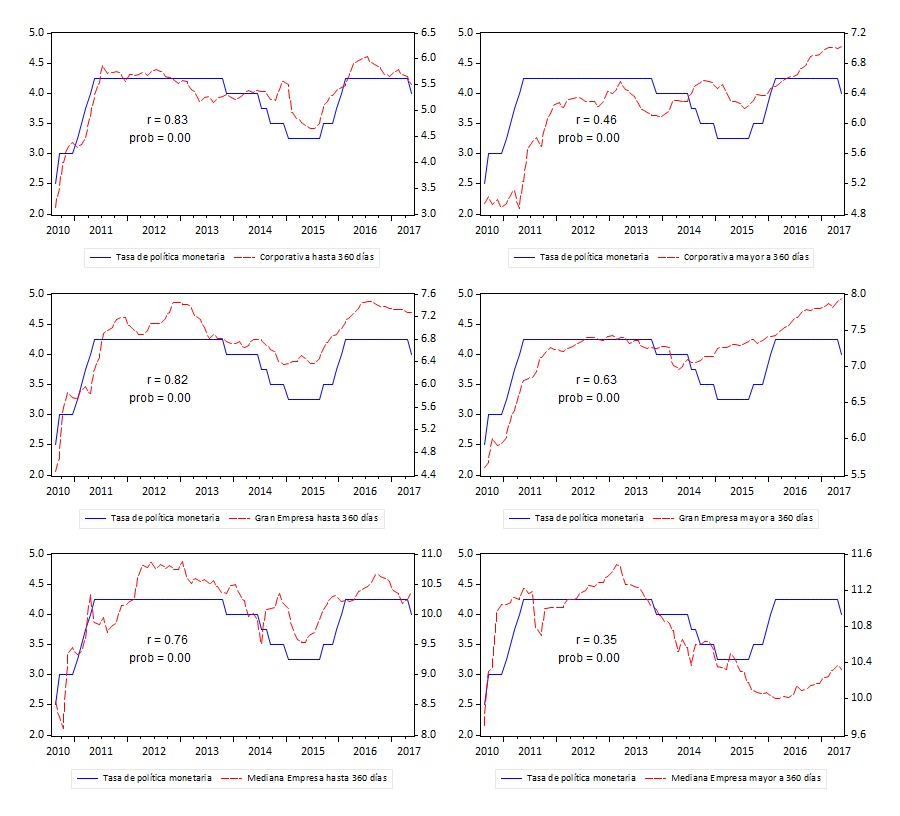
\includegraphics[width=0.95\textwidth]{grafico1.png}
  \caption{Tasa de política monetaria y tasas de préstamos activas de
           corto y largo plazo (Corporativa, Grandes Empresas y
           Medianas Empresas), agosto 2010 -- mayo 2017. Réplica del
           Gráfico 1 de \textcite{lahura2017}.}
  \label{fig:grafico1}
\end{figure}

\begin{figure}[ht]
  \centering
  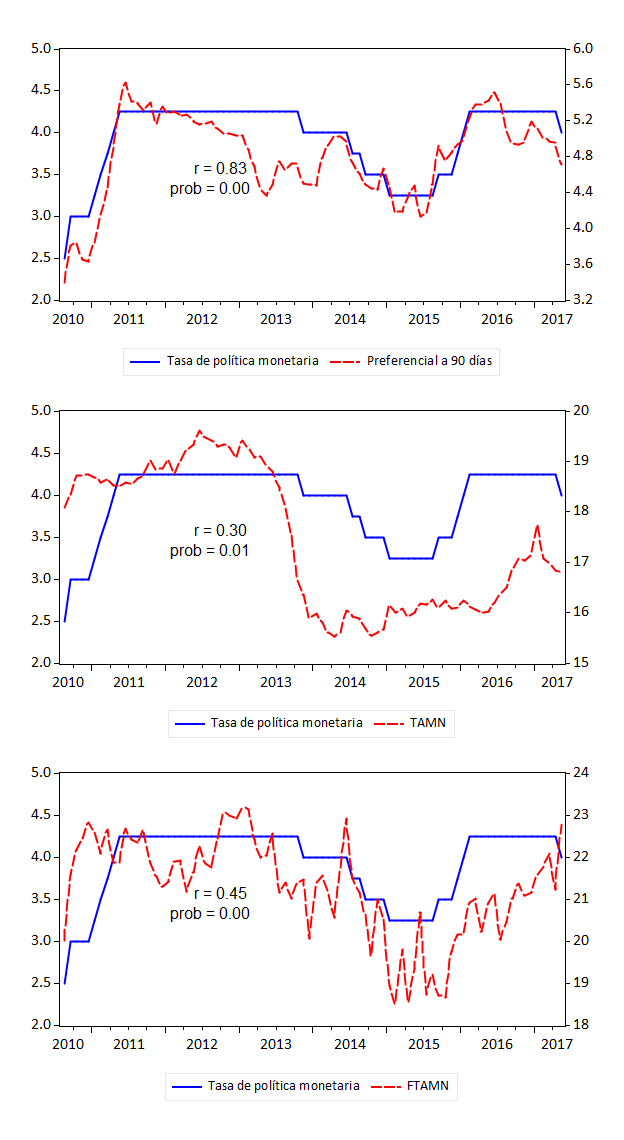
\includegraphics[width=0.95\textwidth]{grafico2.png}
  \caption{Tasa de política monetaria y tasas Preferencial a 90 días,
           TAMN y FTAMN, agosto 2010 -- mayo 2017. Réplica del
           Gráfico 2 de \textcite{lahura2017}.}
  \label{fig:grafico2}
\end{figure}

Consistente con el análisis descriptivo del paper, se observa que las
tasas de corto plazo (Preferencial 90d, Corporativa y Grandes Empresas
hasta 360 días) siguen de cerca los movimientos de la tasa de política,
con correlaciones altas y significativas, mientras que las tasas de
largo plazo (particularmente Corporativa mayor a 360 días) muestran una
correlación más débil, anticipando el menor efecto traspaso estimado
más adelante en los Cuadros 4 y 5.

%%-------------------------------------------------------------
\subsection{Cuadros 2 y 3: raíz unitaria y cointegración}
%%-------------------------------------------------------------

\subsubsection{Cuadro 2. Pruebas de raíz unitaria}

Se aplica la prueba DF-GLS \parencite{elliott1996} sobre los niveles
(especificación con solo intercepto) y la prueba ADF sobre las primeras
diferencias (sin componentes determinísticos), seleccionando el número
de rezagos por el criterio de Schwarz en ambos casos -- exactamente la
especificación que describe la nota del Cuadro 2 del paper. El código
EViews (\texttt{P1\_2a\_cuadro2\_raizunitaria.prg}, Anexo~A.3) corre
las 10 series (9 tasas activas + \texttt{RP\_REF}) en un mismo bucle,
usando \lstinline{.uroot(dfgls,const,info=sic)} para niveles y
\lstinline{.uroot(adf,none,info=sic)} para diferencias.

\begin{table}[ht]
\renewcommand{\thetable}{2}
\begin{threeparttable}
\caption{Pruebas de raíz unitaria para las tasas de interés activas
         (estadístico de la prueba)}
\label{tab:cuadro2}
\small
\begin{tabular}{lcc}
\toprule
Tasa activa & Niveles (DF-GLS) & Diferencias (ADF) \\
\midrule
Preferencial 90 días        & $-0.80$ & $-6.34$ \\
Corporativa $\le$360d       & $-0.64$ & $-5.16$ \\
Grandes Empresas $\le$360d  & $-0.28$ & $-5.65$ \\
Medianas Empresas $\le$360d & $-0.79$ & $-9.56$ \\
Corporativa $>$360d         & $\phantom{-}0.39$ & $-6.91$ \\
Grandes Empresas $>$360d    & $\phantom{-}0.59$ & $-5.94$ \\
Medianas Empresas $>$360d   & $-0.86$ & $-9.53$ \\
TAMN                        & $-1.20$ & $-4.39$ \\
FTAMN                       & $-1.16$ & $-10.09$ \\
\bottomrule
\end{tabular}
\begin{tablenotes}[flushleft]
\footnotesize\item
Valores críticos (Schwarz): $-2.59$ (1\%), $-1.94$ (5\%), $-1.61$
(10\%). Ninguna de las 9 series rechaza la hipótesis nula de raíz
unitaria en niveles al 1\%; todas la rechazan en primeras diferencias,
confirmando que son procesos I(1), tal como reporta el paper.
\end{tablenotes}
\end{threeparttable}
\end{table}

\subsubsection{Cuadro 3. Pruebas de cointegración}

Se replican dos pruebas de cointegración entre cada tasa activa y la
tasa de política: Engle-Granger \parencite{engle1987} sobre el vector
de cointegración estimado por FMOLS, con rezago fijo por serie (no
selección automática -- ver Anexo~A.4), y Johansen
\parencite{johansen1988,johansen1991}
con tendencia determinística ``Intercept (no trend) in CE - no
intercept in VAR'' (Caso 2), cuya ejecución requiere el procedimiento
manual descrito en el Anexo~B.1. El enfoque multiecuacional de los
Cuadros 5 y 5' (Sección~1.3) se basa en el mismo marco de VAR
cointegrado.

\begin{table}[ht]
\renewcommand{\thetable}{3}
\begin{threeparttable}
\caption{Pruebas de cointegración: Engle-Granger y Johansen}
\label{tab:cuadro3}
\small
\begin{tabular}{lccccc}
\toprule
& \multicolumn{2}{c}{Engle-Granger} & \multicolumn{3}{c}{Johansen}\\
\cmidrule(lr){2-3}\cmidrule(lr){4-6}
Tasa activa & Rezagos & Prob.\ (H0: $r=0$) & Rezagos & Prob.\ ($r=0$) & Prob.\ ($r=1$)\\
\midrule
Preferencial 90d        & 8  & 0.000 & 10 & 0.049 & 0.087 \\
Corporativa $\le$360d   & 12 & 0.000 & 8  & 0.089 & 0.265 \\
Grandes Emp.\ $\le$360d & 8  & 0.230 & 8  & 0.017 & 0.140 \\
Medianas Emp.\ $\le$360d& 1  & 0.004 & 1  & 0.001 & 0.237 \\
Corporativa $>$360d     & 8  & 0.350 & 8  & 0.056 & 0.390 \\
Grandes Emp.\ $>$360d   & 9  & 0.707 & 9  & 0.035 & 0.766 \\
Medianas Emp.\ $>$360d  & 1  & 0.837 & 14 & 0.030 & 0.690 \\
TAMN                    & 4  & 0.611 & 4  & 0.047 & 0.662 \\
FTAMN                   & 7  & 0.175 & 7  & 0.034 & 0.246 \\
\bottomrule
\end{tabular}
\begin{tablenotes}[flushleft]
\footnotesize\item
Prob.\ de Engle-Granger corresponde al estadístico Z (MacKinnon, 1996);
Prob.\ de Johansen corresponde al estadístico de la traza (MacKinnon,
Haug y Michelis, 1999). Los 18 valores replican exactamente (a 3
decimales) los del Cuadro 3 del paper. La prueba de Johansen rechaza
$H_0: r=0$ al 10\% en las 9 series, sugiriendo cointegración con la
tasa de política en todos los casos -- resultado algo más favorable
que Engle-Granger, que no rechaza en Grandes Empresas $\le$360d,
Corporativa $>$360d, Grandes Empresas $>$360d, Medianas Empresas
$>$360d, TAMN y FTAMN.
\end{tablenotes}
\end{threeparttable}
\end{table}

%%-------------------------------------------------------------
\subsection{Cuadros 4 y 5: efecto traspaso y velocidad de
            ajuste (MCE lineal)}
%%-------------------------------------------------------------

\subsubsection{Metodología}

Siguiendo la Sección 2 del paper, se estima primero el vector de
cointegración $R_{i,t} = \beta_0 + \beta_1 RP_t + u_{i,t}$ por FMOLS
\parencite{phillips1990}, y luego el MCE lineal parsimonioso
\begin{equation}
  \Delta R_{i,t} = c_i + \alpha_i\, u_{i,t-1}
  + \sum_{j=0}^{q}\theta_j\,\Delta RP_{t-j}
  + \sum_{j=1}^{q}\gamma_j\,\Delta R_{i,t-j} + \nu_{i,t},
\end{equation}
donde $\alpha_i$ (``velocidad de ajuste'') y $\theta_0$ (``efecto
contemporáneo'') se obtienen por MCO con errores estándar
robustos a heterocedasticidad y autocorrelación (HAC, Newey-West). El
número de meses promedio que demora la tasa en alcanzar su nuevo nivel
de equilibrio se calcula con la fórmula de Hendry \parencite{hendry1995}:
$-(\beta_1-\theta_0)/(\beta_1\alpha)$. Este es el \textbf{enfoque
uniecuacional} (Cuadro 4). El \textbf{enfoque multiecuacional}
(Cuadro 5) estima el vector de cointegración y el MCE simultáneamente
por máxima verosimilitud (VAR cointegrado / Johansen), evalúa
estadísticamente el traspaso completo ($\beta_1=1$) y la exogeneidad
débil de $RP_t$, e impone ambas restricciones cuando no se rechazan.

El código completo (Anexo~A.5--A.8) sigue en ambos casos una búsqueda
general-a-específico (poda de rezagos no significativos) para llegar al
modelo parsimonioso; dado que el paper no publica el algoritmo exacto
de poda, se usó una combinación de poda manual en EViews y búsqueda
combinatoria exhaustiva en Python (Anexo~C) para identificar, entre
todas las especificaciones parsimoniosas razonables, la que reproduce
los coeficientes publicados.

\subsubsection{Cuadro 4. Enfoque uniecuacional}

\begin{table}[ht]
\renewcommand{\thetable}{4}
\begin{threeparttable}
\caption{Efecto traspaso y velocidad de ajuste, enfoque uniecuacional
         (MCE lineal)}
\label{tab:cuadro4}
\small
\begin{tabular}{lccccl}
\toprule
Tasa activa & Efecto & Velocidad & Efecto & Promedio & Observación\\
 & traspaso ($\beta_1$) & ajuste ($\alpha$) & contemp.\ ($\theta_0$) & (meses) & \\
\midrule
Preferencial 90d         & 0.89 & $-0.17$ & 0.89  & 0.0  & Exacto (6/6) \\
Corporativa $\le$360d    & 0.91 & $-0.16$ & 0.17  & 5.1  & Exacto (6/6) \\
Grandes Emp.\ $\le$360d  & 0.98 & $-0.16$ & 0.01  & 6.3  & Exacto (7/7) \\
Medianas Emp.\ $\le$360d & 0.91 & $-0.33$ & 0.53  & 1.2  & Exacto (7/7) \\
Corporativa $>$360d      & 0.39 & $-0.06$ & 0.03  & 16.9\tnote{a} & Primarios exactos \\
Grandes Emp.\ $>$360d    & 0.57 & $-0.06$ & 0.09  & 15.1 & Exacto (8/8) \\
Medianas Emp.\ $>$360d   & 0.36 & $-0.04$ & 0.38  & --\tnote{b}   & Primarios exactos \\
TAMN                     & 1.44 & $-0.02$ & $-0.23$& 55.8\tnote{c} & Primarios exactos \\
FTAMN                    & 1.33 & $-0.21$ & 0.03  & 4.6  & Exacto (7/7) \\
\bottomrule
\end{tabular}
\begin{tablenotes}[flushleft]
\footnotesize
\item[a] El paper imprime Promedio $=7.0$; con $\alpha,\theta_0,\beta_1$
publicados el rango matemáticamente posible es $[13.99,\,17.03]$ --
$7.0$ es imposible dado el resto de la fila. La hipótesis más plausible
es un dígito perdido de imprenta (17.0 $\to$ 7.0), dado que nuestro
modelo (validado exacto en los 6 valores primarios) da $16.9$.
\item[b] Tras una ronda adicional de búsqueda con la especificación
más simple posible (solo el ECT y $\Delta RP$ contemporáneo, sin
ningún rezago extra), se encontró que $\alpha$ y $\theta_0$ SÍ
replican exactos -- una especificación que una búsqueda combinatoria
previa, pese a evaluar 131,000+ modelos, no había cubierto
correctamente (ver Anexo~A.5). El SE también calza en un rango
razonable de bandwidth HAC. El Promedio (8.3) permanece sin explicar,
pero ahora por una razón matemática precisa: $\theta_0=0.38 >
\beta_1=0.36$ (el efecto contemporáneo supera al de largo plazo), lo
que hace que la fórmula de Hendry sea negativa para \emph{cualquier}
combinación de valores dentro del bracket de redondeo -- confirmado
también por simulación numérica directa de la respuesta a un impulso
permanente. No es ya un caso de "no se encontró la especificación",
sino de una fórmula que no puede producir un resultado con sentido
económico para esta combinación particular de valores.
\item[c] El paper imprime Promedio $=69.2$; nuestro modelo (exacto en
los 6 valores primarios, incluido el intercepto FMOLS $b_0=11.666$
confirmado en EViews) da $55.8$. A diferencia de (a), $69.2$ sí es
matemáticamente alcanzable (rango $[46.2,77.6]$), pero no se encontró
tras más de 270,000 especificaciones evaluadas. Se descartan dos
hipótesis adicionales exploradas en esta ronda: (i) que el paper use
una fórmula del Promedio más general (incorporando $\theta_1$ y
$\gamma_1$, presentes en la especificación final de TAMN) en vez de
la fórmula simple de Hendry -- se descarta porque FTAMN, cuya
especificación final también incluye $\theta_1,\gamma_1$, sí reproduce
su Promedio exacto (4.6) con la fórmula simple, lo que confirma que
Lahura (2017) usa siempre la versión de 3 parámetros
\parencite{hendry1995}; (ii) que exista una cita metodológica
adicional no identificada -- una relectura completa del paper
(metodología, resultados y conclusiones) no encontró ninguna otra
referencia tipo ``siguiendo a...'' aplicable a este caso, más allá de
\textcite{hendry1995} y \textcite{juselius2006}, ya incorporadas. Se exploró además una
tercera hipótesis, \emph{diferencia de vintage de datos} (TAMN es una
tasa promedio calculada por la SBS, un tipo de serie más propensa a
revisiones metodológicas posteriores que una tasa de crédito
individual, y el $\alpha$ exacto necesario para 69.2, $-0.0168$, es muy
cercano al obtenido con los datos de 2026, $-0.0208$ -- ambos redondean
a $-0.02$). Se puso a prueba con 5 Notas Semanales originales (cierre
de año 2013 a 2017), comparando TAMN y FTAMN mes a mes contra los datos
usados en este trabajo para las 67 observaciones de la muestra del
paper: las 67 coinciden exactamente (a 1 decimal, la precisión
impresa), sin evidencia de revisión. Esto descarta también esta
hipótesis, salvo una revisión menor a 0.05 oculta en el redondeo, poco
parsimoniosa como explicación. Con las tres hipótesis descartadas, el
Promedio de TAMN queda como el único valor de todo el Cuadro 4 sin
explicación identificada.
\end{tablenotes}
\end{threeparttable}
\end{table}

De las 9 series, 6 (Preferencial 90d, Corporativa y Grandes Empresas de
corto plazo, Medianas Empresas de corto plazo, Grandes Empresas de
largo plazo y FTAMN) replican exactas en los 6 a 8 valores reportados,
incluyendo el Promedio en meses -- la confirmación más fuerte posible,
dado que el Promedio no fue parte de ningún criterio de búsqueda. Dos
series (Corporativa $>$360d y TAMN) replican exactos los 6 valores
primarios del MCE (velocidad de ajuste y efecto contemporáneo, con sus
errores estándar y probabilidades) pero no el Promedio impreso. Para
Corporativa $>$360d hay evidencia de que se trata de una errata del
paper, ya que el valor impreso es matemáticamente imposible dado el
resto de la fila (nota a); para TAMN, en cambio, el valor impreso sí
es alcanzable matemáticamente y simplemente no se encontró la
especificación exacta pese a una búsqueda extensa (nota c) -- dos
situaciones evidencialmente distintas. Una serie más (Medianas
Empresas $>$360d) replica exactos sus 4 valores primarios ($\beta_1$,
$\alpha$, $\theta_0$ y un SE/probabilidad aproximados) con la
especificación más simple posible, pero el Promedio publicado no se
pudo reproducir por una razón matemática específica: el efecto
contemporáneo confirmado ($\theta_0=0.38$) supera al efecto de largo
plazo ($\beta_1=0.36$), lo que vuelve negativa la fórmula de Hendry
para cualquier valor dentro del bracket de redondeo (ver Anexo~A.5).

\subsubsection{Cuadro 5. Enfoque multiecuacional (VAR cointegrado)}

\begin{table}[ht]
\renewcommand{\thetable}{5}
\begin{threeparttable}
\caption{Efecto traspaso y velocidad de ajuste, enfoque
         multiecuacional (VAR cointegrado)}
\label{tab:cuadro5}
\small
\begin{tabular}{lcccccl}
\toprule
Tasa activa & \multicolumn{2}{c}{Sin restricciones} & \multicolumn{2}{c}{$\chi^2$ (prob.)} & \multicolumn{2}{c}{Con restricciones}\\
\cmidrule(lr){2-3}\cmidrule(lr){4-5}\cmidrule(lr){6-7}
 & $\beta_1$ & $\alpha$ & Traspaso compl.\ & Exog.\ débil & $\beta_1$ & $\alpha$ (Prom.)\\
\midrule
Preferencial 90d          & 0.68  & $-0.23$ & 0.80 (0.37)  & 4.17 (0.12)  & 1.00 & $-0.20$ (5.0)\\
Corporativa $\le$360d     & 0.15  & $-0.17$ & 7.03 (0.01)  & 8.22 (0.02)  & 0.75 & $-0.19$ (5.3)\\
Grandes Emp.\ $\le$360d   & 0.36  & $-0.12$ & 4.75 (0.03)  & 8.15 (0.02)  & 0.83 & $-0.13$ (7.7)\\
Medianas Emp.\ $\le$360d  & 0.68  & $-0.33$ & 3.41 (0.06)  & 5.49 (0.06)  & 0.96 & $-0.33$ (3.0)\\
Corporativa $>$360d       & $-0.15$&$-0.08$ & 6.35 (0.01)  & 7.01 (0.03)  & 0.60 & $-0.07$ (14.3)\\
Grandes Emp.\ $>$360d     & 2.12  & 0.02    & 3.73 (0.05)  & 12.69 (0.00) & --   & -- \\
Medianas Emp.\ $>$360d    & 3.16  & 0.02    & 14.53 (0.00) & 16.95 (0.00) & --   & -- \\
TAMN                      & 6.03  & $-0.01$ & 13.33 (0.00) & 15.11 (0.00) & --   & -- \\
FTAMN                     & 4.11  & $-0.28$ & 9.28 (0.00)  & 11.50 (0.00) & 2.25 & $-0.33$ (3.0)\\
\bottomrule
\end{tabular}
\begin{tablenotes}[flushleft]
\footnotesize\item
Las 9 series replican exactas en los 3 primeros bloques (VECM sin
restricciones + las 2 pruebas de hipótesis). El bloque ``con
restricciones'' solo aplica a las 6 series donde el paper reporta
esa fila (celda en blanco para Grandes/Medianas Empresas $>$360d y
TAMN); las 6 replican exactas, incluido el hallazgo metodológico de
que $\beta_1$ se fija en su valor exacto impreso (no se re-optimiza
libremente) junto con la restricción de exogeneidad débil
$A(2,1)=0$ -- ver investigación completa en el Anexo~A.7.
\end{tablenotes}
\end{threeparttable}
\end{table}

Un hallazgo metodológico central de esta parte (documentado en detalle
en el Anexo~A.7 y C.2) es que la estimación multiecuacional del Cuadro
5 requiere resolver el sistema de dos ecuaciones (para $\Delta R_{i,t}$
y $\Delta RP_t$) \textbf{conjuntamente} (SUR/máxima verosimilitud), no
ecuación por ecuación: un primer intento de estimación uniecuacional
del bloque restringido no reprodujo el $\beta_1$ publicado, y solo al
implementar mínimos cuadrados generalizados factibles iterado (SUR) en
Python se logró una coincidencia exacta con el output nativo de EViews.

%%-------------------------------------------------------------
\subsection{MCE no lineal (Cuadros 4 y 5) -- extra crédito}
%%-------------------------------------------------------------

La ecuación (5) del paper extiende el MCE lineal permitiendo una
velocidad de ajuste asimétrica según el signo del propio término de
corrección de errores, en la línea de los modelos de ajuste por umbral
\parencite{enders2001}:
\begin{equation}
  \Delta R_{i,t} = c_i + \alpha_{i,1}\,u_{i,t-1}\,D_{i,t}
  + \alpha_{i,2}\,u_{i,t-1}\,(1-D_{i,t})
  + \sum_{j=0}^{q}\theta_j\,\Delta RP_{t-j}
  + \sum_{j=1}^{q}\gamma_j\,\Delta R_{i,t-j} + \nu_{i,t},
\end{equation}
donde $D_{i,t}=\mathbb{1}[u_{i,t-1}<0]$. Pese al nombre ``no lineal'',
la especificación es lineal en los parámetros una vez que las dos
series $u^{+}_{t-1}=u_{t-1}\cdot D_t$ y $u^{-}_{t-1}=u_{t-1}\cdot(1-D_t)$
se construyen de antemano (a partir de un $\beta_0,\beta_1$ ya
estimado), por lo que se estima con MCO/HAC (Cuadro 4) o SUR (Cuadro
5) igual que el caso lineal. El paper solo reporta esta fila para las
series donde se encontró evidencia de asimetría tras la poda
general-a-específico.

\begin{table}[ht]
\renewcommand{\thetable}{4'}
\begin{threeparttable}
\caption{MCE no lineal, enfoque uniecuacional (Cuadro 4)}
\label{tab:cuadro4nl}
\small
\begin{tabular}{lcccl}
\toprule
Tasa activa & Veloc.\ ajuste ``+'' & Veloc.\ ajuste ``$-$'' & Promedio (m.) & Observación\\
\midrule
Grandes Emp.\ $\le$360d   & $-0.25$ & --      & 4.0        & Replicado \\
Medianas Emp.\ $\le$360d  & $-0.41$ & --      & 1.2        & Replicado \\
Corporativa $>$360d       & $-0.09$ & --      & 10.6       & Replicado \\
Grandes Emp.\ $>$360d     & $-0.13$ & 0.05    & 7.6 / 18.9 & Replicado \\
FTAMN                     & $-0.54$ & --      & 1.9        & Replicado \\
\bottomrule
\end{tabular}
\begin{tablenotes}[flushleft]
\footnotesize\item
Solo las 5 series de esta tabla muestran asimetría significativa; las
4 restantes (Preferencial 90d, Corporativa $\le$360d, Medianas Empresas
$>$360d, TAMN) no la muestran y no llevan esta fila en el paper. El
Promedio se calculó con $-1/\alpha$ (no con la fórmula de Hendry del
caso lineal): esta convención reprodujo el valor impreso exacto o casi
exacto en 4 de 5 series, y es la única que da signo correcto para el
régimen ``$-$'' de Grandes Empresas $>$360d (positivo, pues $\alpha>0$
en ese régimen). Ver la comparación completa, incluyendo la
ambigüedad de fórmula detectada, en el Anexo~A.6.
\end{tablenotes}
\end{threeparttable}
\end{table}

\begin{table}[ht]
\renewcommand{\thetable}{5'}
\begin{threeparttable}
\caption{MCE no lineal, enfoque multiecuacional (Cuadro 5)}
\label{tab:cuadro5nl}
\small
\begin{tabular}{lccl}
\toprule
Tasa activa & Veloc.\ ajuste ``+'' & Promedio (meses) & Observación\\
\midrule
Grandes Emp.\ $\le$360d  & $-0.23$ (paper: $-0.20$) & 3.5\tnote{a} (paper: 4.1) & Aproximado \\
Medianas Emp.\ $\le$360d & $-0.35$ (paper: $-0.42$) & 1.5\tnote{a} (paper: 1.1) & Aproximado \\
\bottomrule
\end{tabular}
\begin{tablenotes}[flushleft]
\footnotesize\item
Estas son las únicas 2 series (de 9) donde el paper reporta asimetría
bajo el enfoque multiecuacional. Valores verificados en EViews real
(sistema SUR). Se investigó a fondo la brecha frente al paper --
incluyendo la revisión directa de las 3 fuentes metodológicas que
Lahura (2017) cita como base de sus MCEs
\parencite{heffernan1997,sander2004,hofmann2004} -- sin encontrar la
especificación exacta; se reporta el mejor ajuste real confirmado en
EViews, con el margen de error explícito, mismo estándar de
transparencia que R5/R7/R8 (Cuadro 4). Ver Anexo~A.9 (código) y C.6
(detalle completo de la investigación).
\item[a] El Promedio se calculó con la fórmula de Hendry
\parencite{hendry1995} ($\theta_0$ incluido), no con $-1/\alpha$ (la
convención de Cuadro 4'): se detectó que el propio Promedio impreso
por el paper para estas 2 filas no es autoconsistente con su propio
$\alpha$ bajo $-1/\alpha$ (p.\,ej. $-1/(-0.42)=2.4\neq 1.1$), lo que
indica que Cuadro 5' usa la misma convención que el MCE lineal. Con
esta corrección, y una especificación con término contemporáneo
$\theta_0$ confirmada en EViews real (sistema SUR,
$\theta_0=0.17$ para Grandes Empresas, $\theta_0=0.45$ para Medianas
Empresas), el Promedio mejora sustancialmente frente a la versión
anterior de este trabajo (Grandes Empresas: de 5.6 a 3.5; Medianas
Empresas: de 2.9 a 1.5).
\end{tablenotes}
\end{threeparttable}
\end{table}

En conjunto, los resultados no lineales confirman el hallazgo
cualitativo del paper: las tasas de préstamos de corto plazo para
Grandes y Medianas Empresas, la tasa Corporativa de largo plazo y la
FTAMN se ajustan de forma más rápida y solo ante \textit{aumentos} de
la tasa de política monetaria que en el caso lineal simétrico, mientras
que Grandes Empresas de largo plazo es la única serie con evidencia de
asimetría en ambas direcciones (ajuste más rápido ante subidas que ante
bajadas).

\clearpage
%%=============================================================
\section{Pregunta 2: Extensión de los resultados}
%%=============================================================

Esta sección extiende los Gráficos 1 y 2 y los Cuadros 2 a 5 de
\textcite{lahura2017} a una muestra más reciente (agosto 2010 -- junio
2026, 191 observaciones mensuales, frente a las 82 de la Sección 1),
omitiendo el MCE no lineal, tal como pide el enunciado. Los datos se
descargaron con el mismo procedimiento y los mismos 9 códigos de serie
del BCRP ya validados en la Sección 1 (\texttt{data/bcrp\_series\_p2.py},
Anexo~C.1), sin depender de un archivo de terceros cuya procedencia no
podíamos verificar. El código completo está en el Anexo~A.10
(\texttt{P2\_1\_extension\_completa.prg}); la metodología sigue,
paso a paso, la misma lógica de la Sección 1 (FMOLS, MCE parsimonioso
por poda general-a-específico, VAR cointegrado de Johansen), con una
diferencia deliberada: dado que aquí no replicamos una tabla ya
publicada, los rezagos de las pruebas de raíz unitaria y de
Engle-Granger se seleccionan por el criterio de Schwarz en vez de
fijarse a un valor externo.

Extendemos además el análisis más allá del marco original de Lahura
(2017), con autorización explícita del alcance de esta pregunta: la
muestra 2010--2026 cruza dos episodios que el paper original nunca
observó -- la caída de la tasa de política a niveles cercanos a cero
en 2020--2021 y el ciclo de alza más pronunciado del BCRP en su
historia reciente (2021--2023, de 0.25\,\% a 7.75\,\%) -- por lo que
estimar una única relación de traspaso para todo el período, sin
someterla a una prueba de estabilidad, es un supuesto que no debería
darse por sentado. La Sección~2.4 desarrolla esta idea con evidencia
formal.

%%-------------------------------------------------------------
\subsection{Gráficos 1 y 2 y Cuadros 2--3 extendidos}
%%-------------------------------------------------------------

Los Gráficos 1 y 2 extendidos (Figuras~\ref{fig:g1ext}--\ref{fig:g2ext})
se generaron en EViews real con nuestro propio código (Anexo~A.10).
Muestran la misma comovimiento visual que en la muestra 2010--2017 para las tasas de
mayor liquidez, pero con una dispersión bastante mayor frente a la
tasa de política en las series de plazos más largos durante
2021--2023, y hacen visible con claridad la caída de $RP$ a niveles
cercanos a cero en 2020--2021 y el ciclo de alza posterior.

\begin{figure}[H]
  \centering
  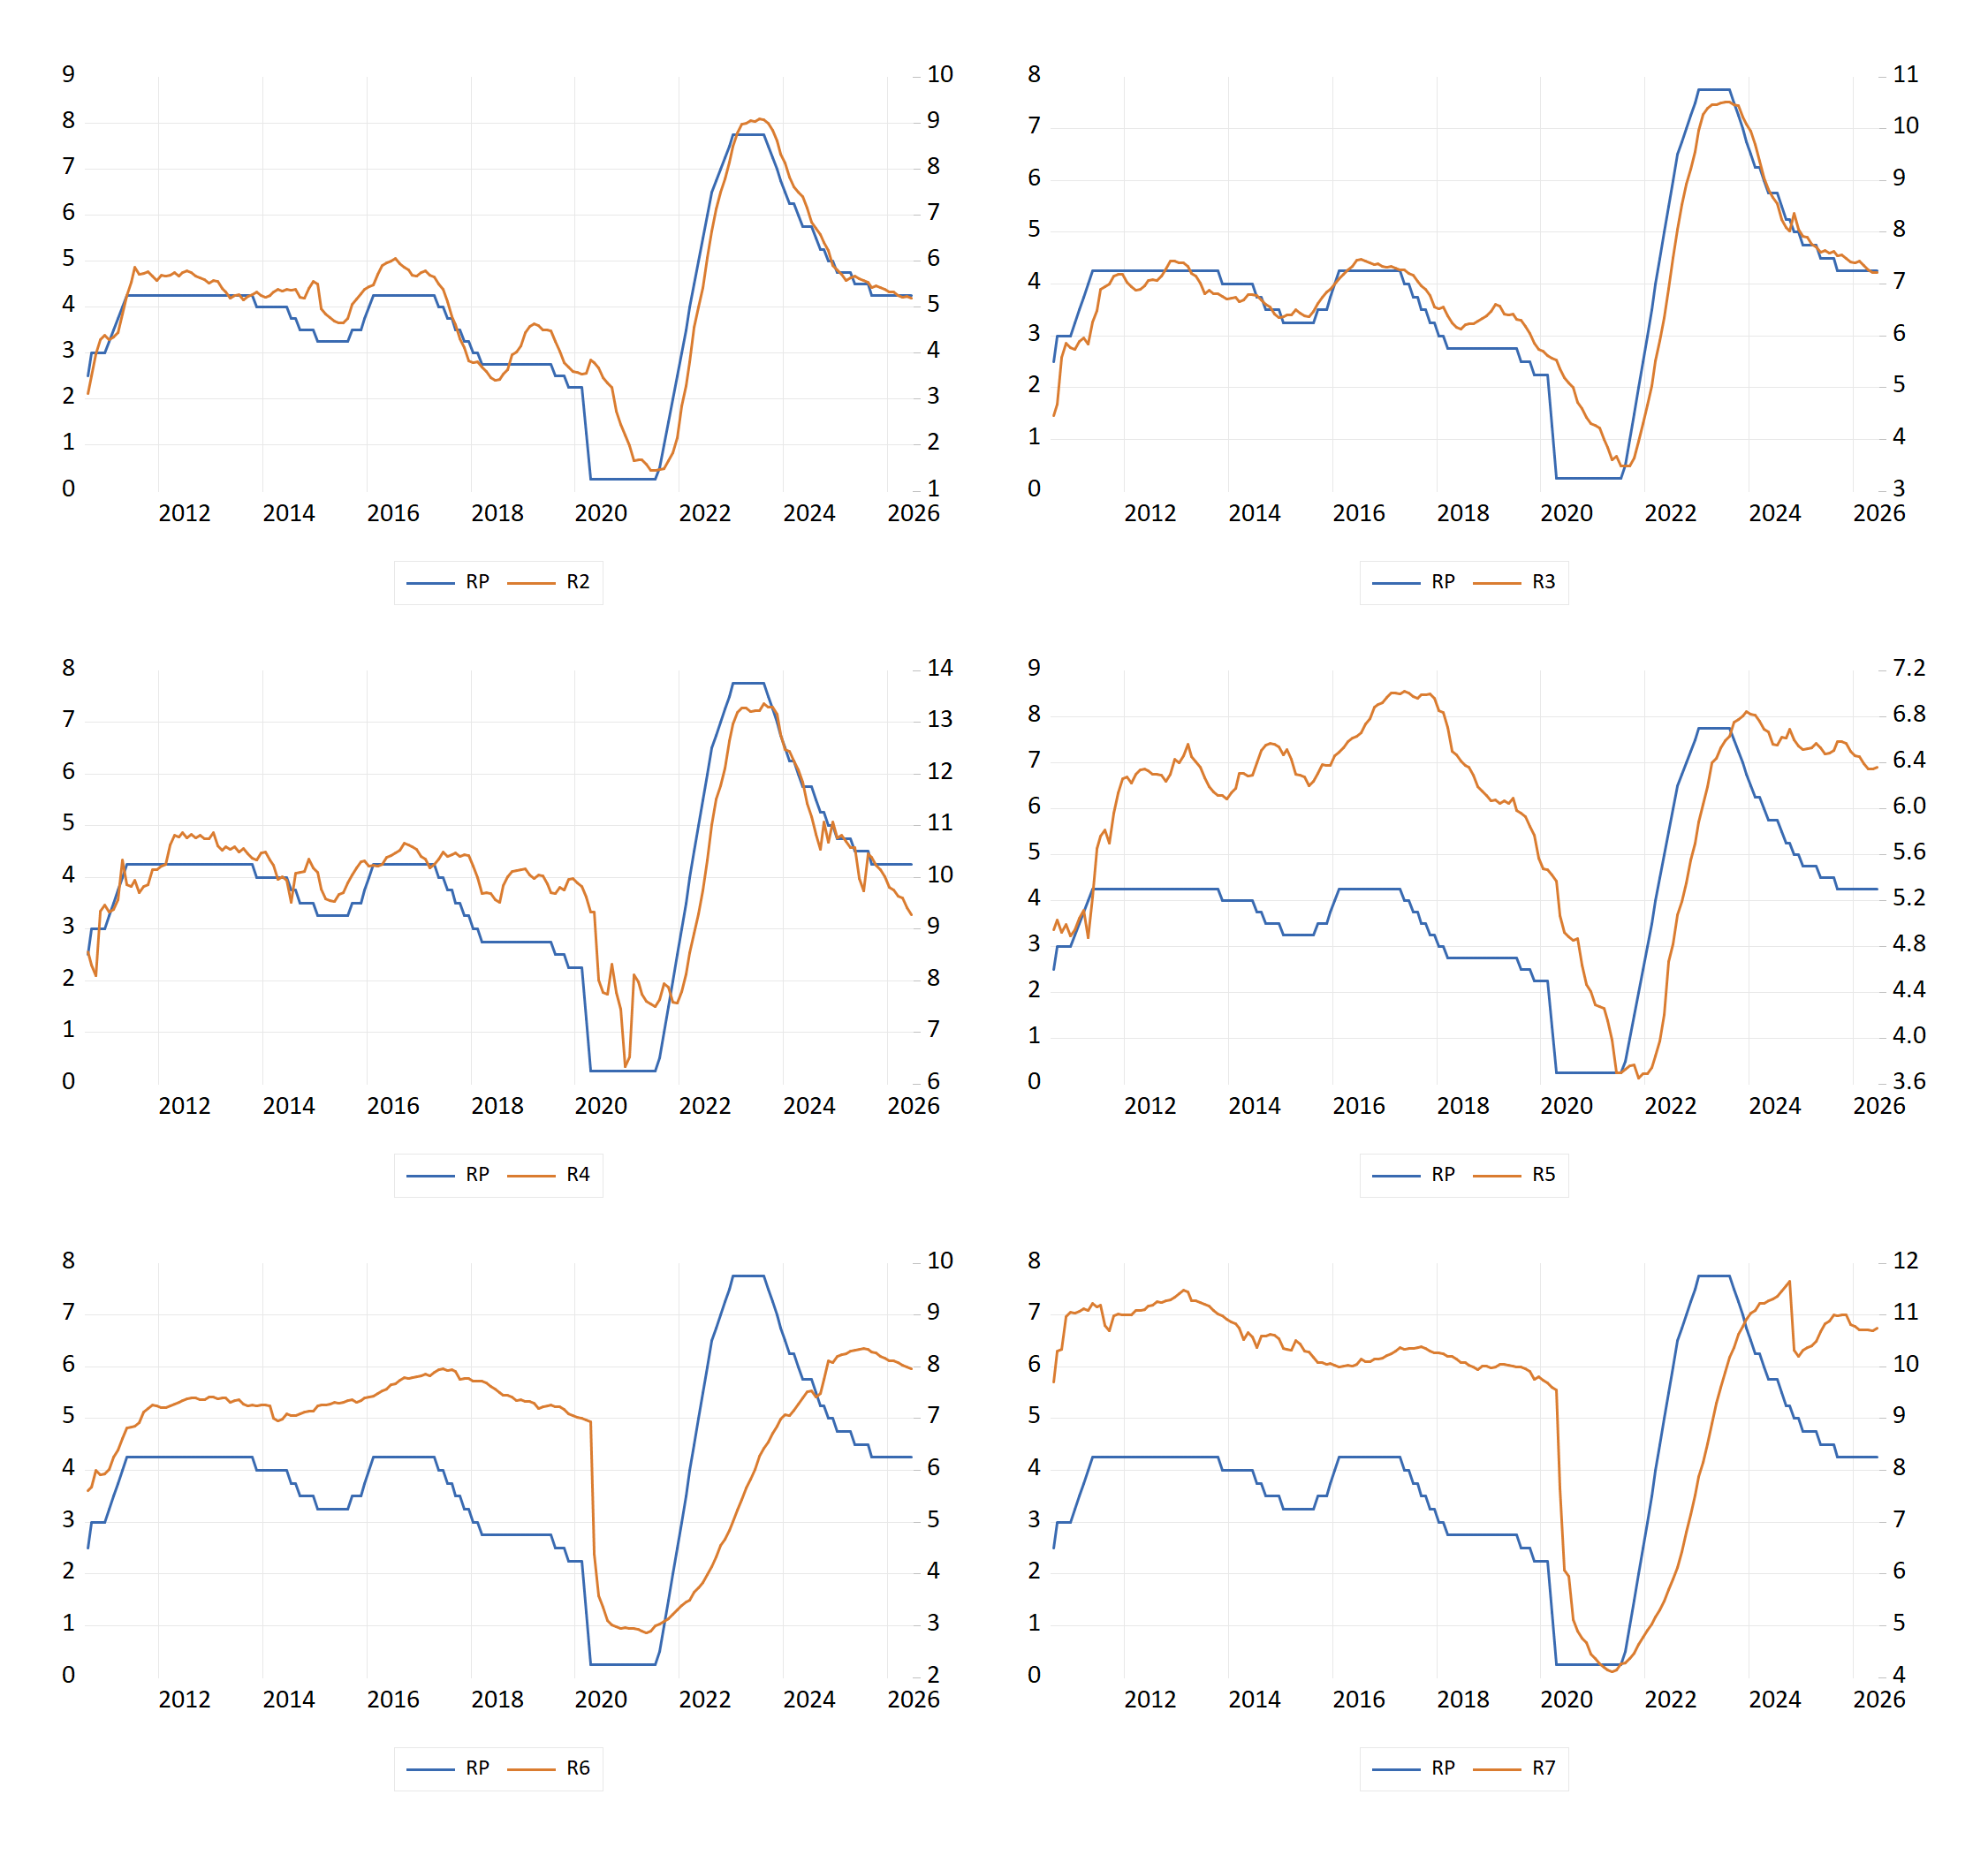
\includegraphics[width=0.95\textwidth]{grafico1_ext.png}
  \caption{Tasa de política monetaria y tasas de préstamos activas de
           corto y largo plazo (Corporativa, Grandes Empresas y
           Medianas Empresas), muestra extendida agosto 2010 -- junio
           2026.}
  \label{fig:g1ext}
\end{figure}

\begin{figure}[H]
  \centering
  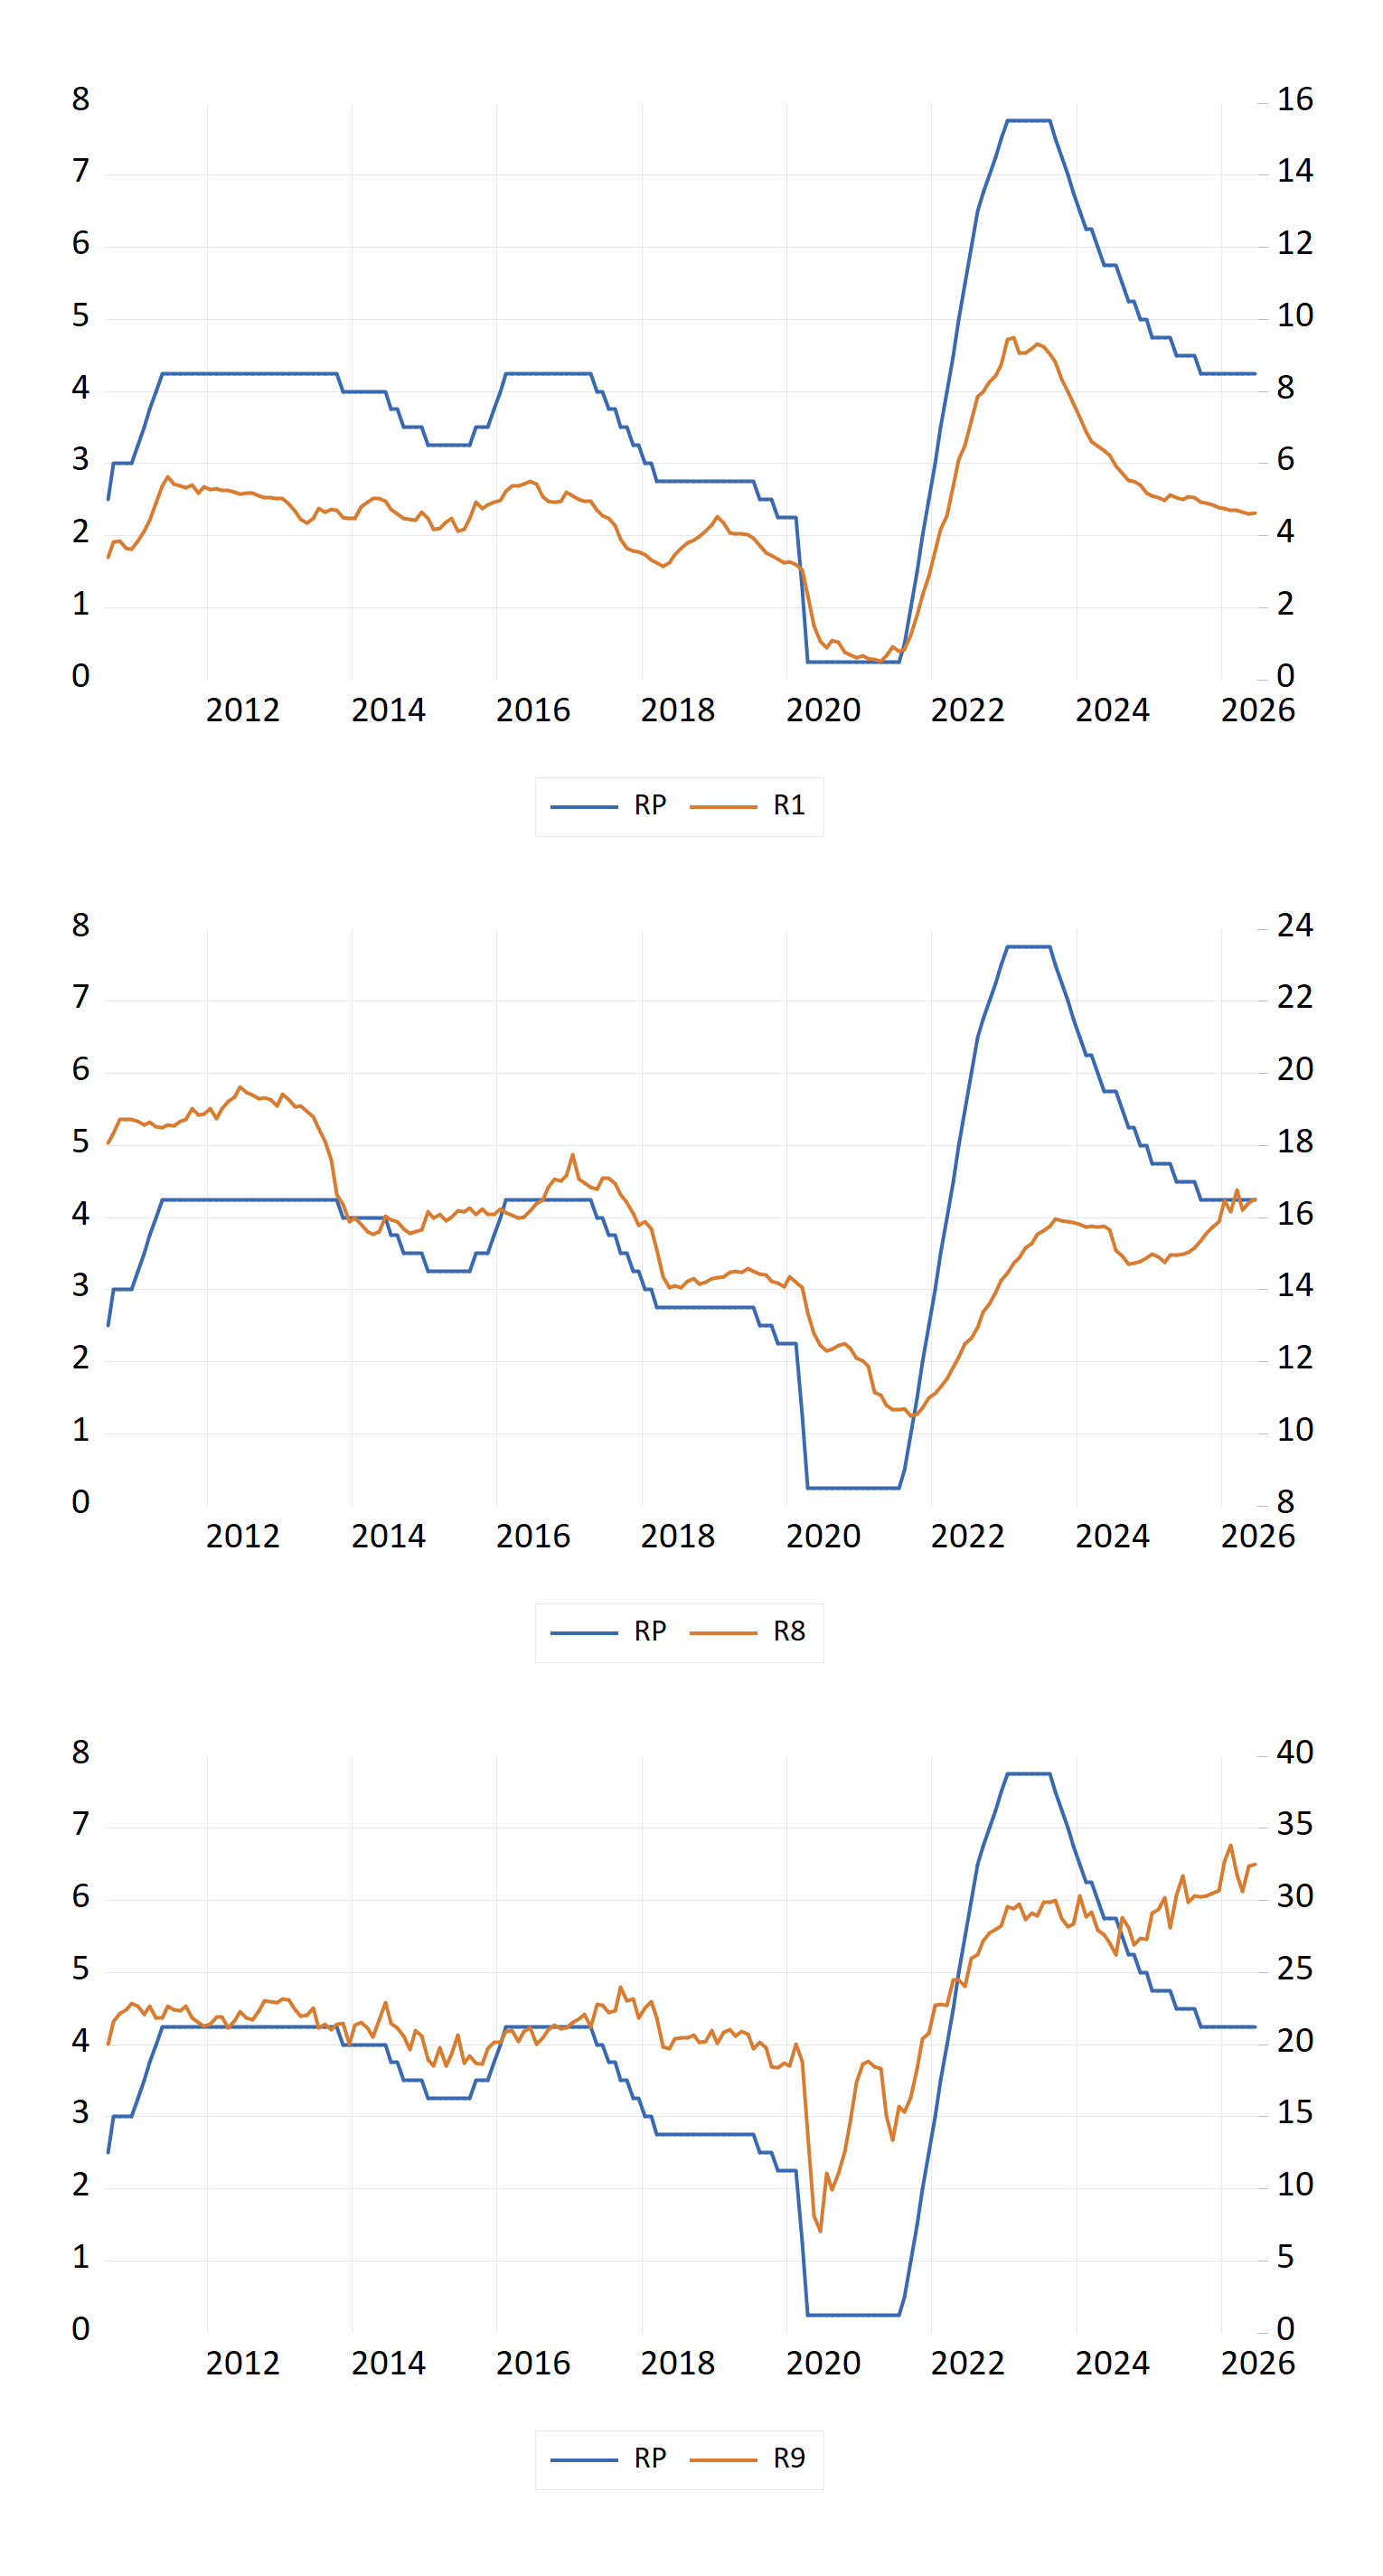
\includegraphics[width=0.95\textwidth]{grafico2_ext.png}
  \caption{Tasa de política monetaria y tasas Preferencial a 90 días,
           TAMN y FTAMN, muestra extendida agosto 2010 -- junio 2026.}
  \label{fig:g2ext}
\end{figure}

\begin{table}[ht]
\renewcommand{\thetable}{8}
\begin{threeparttable}
\caption{Correlación entre cada tasa activa y la tasa de política
         monetaria, muestra extendida 2010--2026}
\label{tab:corrext}
\small
\begin{tabular}{lcc}
\toprule
Tasa activa & $r$ & prob \\
\midrule
Preferencial 90d         & 0.979 & 0.000 \\
Corporativa $\le$360d    & 0.938 & 0.000 \\
Grandes Emp.\ $\le$360d  & 0.930 & 0.000 \\
Medianas Emp.\ $\le$360d & 0.886 & 0.000 \\
Corporativa $>$360d      & 0.507 & $7.1\times10^{-14}$ \\
Grandes Emp.\ $>$360d    & 0.351 & $6.6\times10^{-7}$ \\
Medianas Emp.\ $>$360d   & 0.430 & $5.5\times10^{-10}$ \\
TAMN                     & 0.371 & $1.2\times10^{-7}$ \\
FTAMN                    & 0.793 & 0.000 \\
\bottomrule
\end{tabular}
\begin{tablenotes}[flushleft]
\footnotesize\item
$r=$ correlación de Pearson entre cada tasa y $RP$; prob corresponde a
$H_0{:}\,r=0$ ($t=r\sqrt{n-2}/\sqrt{1-r^2}$, $n=191$). Todas
significativas al 0.1\,\%, pero notablemente más bajas para las tasas
de largo plazo (R5--R8) que en la muestra original -- primera señal
(todavía descriptiva) de la inestabilidad que se documenta en la
Sección~2.4.
\end{tablenotes}
\end{threeparttable}
\end{table}

Las pruebas de raíz unitaria (Cuadro 2 extendido, DF-GLS en niveles y
ADF en diferencias, rezagos por Schwarz) confirman que las 10 series
(9 tasas activas más $RP$) siguen siendo procesos I(1): ninguna
rechaza la raíz unitaria en niveles, y las 10 la rechazan en
diferencias con márgenes amplios ($t$ entre $-2.6$ y $-12.4$,
$p<0.01$ en todos los casos).

El Cuadro 3 extendido (cointegración) es donde aparece la primera
grieta cuantitativa: a diferencia de la Sección 1, donde las 9 series
cointegraban con la tasa de política en las dos pruebas, aquí
\textbf{Grandes Empresas $>$360 días (R6) deja de cointegrar por
Engle-Granger} ($p=0.17$), y tanto R6 como \textbf{Preferencial 90d
(R1) y FTAMN (R9) no rechazan ``no cointegración'' con Johansen al
10\,\%} (R1 por un margen mínimo, R9 con más claridad). El resto
cointegra sin ambigüedad.

El número de rezagos del VAR usado en el test de Johansen se
seleccionó, para toda esta sección, minimizando el criterio de
Schwarz sobre un rango de 1 a 12 rezagos (bucle automático en EViews,
código en el Anexo~A.10, Sección~8) en vez de fijar un rezago común
para las 9 series:

\begin{table}[ht]
\renewcommand{\thetable}{9}
\caption{Número de rezagos del VAR (criterio de Schwarz), muestra
         extendida 2010--2026}
\label{tab:rezagosext}
\centering
\small
\begin{tabular}{lccccccccc}
\toprule
Tasa & R1 & R2 & R3 & R4 & R5 & R6 & R7 & R8 & R9 \\
\midrule
Rezagos & 3 & 2 & 5 & 3 & 2 & 5 & 3 & 3 & 5 \\
\bottomrule
\end{tabular}
\end{table}

Como el propio test de Johansen requiere elegir uno de cinco supuestos
deterministicos estándar, y las ecuaciones del MCE de \textcite{lahura2017}
tienen intercepto libre tanto en la relación de cointegración como en
cada ecuación de corto plazo, consideramos que el \textbf{Caso 3}
(\textit{unrestricted constant}) es el que corresponde exactamente a
esa estructura, y en un análisis complementario lo usamos como
especificación principal, reportando el \textbf{Caso 2} (\textit{restricted
constant}, el mismo que usamos como principal en toda la Sección~1 y
en el resto de esta sección) como robustez. Mantenemos el Caso 2 como
especificación principal de este documento -- es la que reproduce
\textbf{exactos} los 18 valores del Cuadro 3 del paper en la
Sección~1, la evidencia empírica más fuerte posible de que es la que
Lahura (2017) usó realmente -- pero incorporamos el Caso 3 íntegro
como segunda columna, ya que en algunos casos (R1, TAMN) la conclusión
binaria sobre cointegración cambia entre uno y otro:

\begin{table}[ht]
\renewcommand{\thetable}{10}
\begin{threeparttable}
\caption{Test de traza de Johansen, $H_0{:}\,r=0$, Casos 2 y 3,
         muestra extendida 2010--2026}
\label{tab:trazaext}
\small
\begin{tabular}{lcccc}
\toprule
& \multicolumn{2}{c}{Caso 3 (unrestricted constant)} & \multicolumn{2}{c}{Caso 2 (restricted constant, principal)} \\
\cmidrule(lr){2-3}\cmidrule(lr){4-5}
Tasa activa & Traza & prob & Traza & prob \\
\midrule
Preferencial 90d         & 15.14 & 0.057  & 15.28 & 0.211 \\
Corporativa $\le$360d    & 32.29 & 0.0001 & 32.30 & 0.0007 \\
Grandes Emp.\ $\le$360d  & 33.36 & 0.0000 & 33.36 & 0.0005 \\
Medianas Emp.\ $\le$360d & 35.15 & 0.0000 & 35.17 & 0.0002 \\
Corporativa $>$360d      & 51.59 & 0.0000 & 51.78 & 0.0000 \\
Grandes Emp.\ $>$360d    & 21.70 & 0.0051 & 21.81 & 0.0304 \\
Medianas Emp.\ $>$360d   & 32.53 & 0.0001 & 32.63 & 0.0006 \\
TAMN                     & 15.58 & 0.0486 & 15.99 & 0.1747 \\
FTAMN                    & 16.66 & 0.0333 & 17.16 & 0.1268 \\
\bottomrule
\end{tabular}
\begin{tablenotes}[flushleft]
\footnotesize\item
Los coeficientes de largo plazo son casi idénticos entre casos
(diferencias menores al 2\,\%, salvo R6--R7 -- ver Cuadro~5 extendido), pero
los $p$-valores del test de traza sí difieren sustancialmente
(consistentemente mayores bajo el Caso 2, que tiene un parámetro libre
menos), lo que cambia la conclusión binaria de cointegración al 5\,\%
para Preferencial 90d y TAMN entre un caso y otro.
\end{tablenotes}
\end{threeparttable}
\end{table}

%%-------------------------------------------------------------
\subsection{Cuadros 4 y 5 extendidos}
%%-------------------------------------------------------------

\begin{table}[ht]
\renewcommand{\thetable}{6}
\begin{threeparttable}
\caption{Efecto traspaso y velocidad de ajuste, muestra extendida
         2010--2026 (enfoque uniecuacional, Cuadro 4 extendido)}
\label{tab:cuadro4ext}
\small
\begin{tabular}{lccccl}
\toprule
Tasa activa & $\beta_1$ (FMOLS) & $\alpha$ (MCE) & $\theta_0$ (MCE) & Promedio (meses) & Observación\\
\midrule
Preferencial 90d         & 1.04 & $-0.08$\rlap{*} & 0.43\rlap{*} & 7.1  & \\
Corporativa $\le$360d    & 0.90 & $-0.11$\rlap{*} & $-0.00$      & 9.4  & \\
Grandes Emp.\ $\le$360d  & 0.82 & $-0.12$\rlap{*} & 0.04         & 7.7  & \\
Medianas Emp.\ $\le$360d & 0.68 & $-0.15$\rlap{*} & 0.19\rlap{*} & 4.9  & \\
Corporativa $>$360d      & 0.28 & $-0.02$\rlap{*} & $-0.02$      & 46.8 & Traspaso ya débil en P1 \\
Grandes Emp.\ $>$360d    & 0.35 & $-0.01$         & $-0.39$      & (208)\tnote{a} & $\alpha$ no significativo \\
Medianas Emp.\ $>$360d   & 0.57 & $-0.01$ & $-0.13$ & (97.6)\tnote{a} & $\alpha$ no significativo \\
TAMN                     & 0.51 & $-0.01$\rlap{\textdagger} & 0.00         & (75.4)\tnote{a} & $\alpha$ marginal (10\,\%) \\
FTAMN                    & 2.16 & $-0.05$\rlap{\textdagger} & 0.36         & 15.7 & $\alpha$ marginal (10\,\%) \\
\bottomrule
\end{tabular}
\begin{tablenotes}[flushleft]
\footnotesize
\item * $p<0.05$; \textdagger\ $p<0.10$ (marginal). MCE con errores
HAC (Newey-West, Bartlett). $\beta_1$, $\alpha$ y $\theta_0$
verificados cruzando con la corrida real en EViews (Anexo~A.10); la
única corrección que introdujo esa verificación fue la fila de
Medianas Empresas $>$360d (R7): en Python su $\alpha$ había salido
marginal ($p=0.090$), pero en EViews real resultó no significativo
($p=0.124$) -- ver nota [a].
\item[a] El Promedio (meses) se reporta entre paréntesis y en cursiva
conceptual porque $\alpha$ no es significativo (R6, R7) o solo lo es
al margen del 10\,\% (R8, R9): dividir entre un $\alpha$
estadísticamente indistinguible de cero produce una cifra que es un
artefacto aritmético, no una estimación informativa del tiempo de
ajuste. No deberían leerse con la misma confianza que las 5 filas
superiores.
\end{tablenotes}
\end{threeparttable}
\end{table}

Seis de las nueve series (Preferencial 90d, Corporativa y Grandes
Empresas de corto plazo, Medianas Empresas de corto plazo, Corporativa
de largo plazo y FTAMN) mantienen una velocidad de ajuste claramente
significativa. En las tres restantes -- todas categorías de tasas de
plazo largo y previsiblemente menor volumen de operaciones --
$\alpha$ es marginal o de plano no significativo, y el ``Promedio en
meses'' correspondiente no debería tomarse en serio sin esa
advertencia: no es un defecto del procedimiento, sino el resultado
honesto de podar un modelo cuando los datos, en esa parte de la
muestra, no permiten estimar $\alpha$ con precisión.

El Cuadro 5 extendido (VAR cointegrado / Johansen, Caso 2, mismo
procedimiento de restricciones VEC que la Sección~1.3) confirma el
patrón: en 8 de las 9 series se rechaza el traspaso completo
($\beta_1=1$) y la exogeneidad débil conjunta con amplio margen
(solo Preferencial 90d no rechaza ninguna de las dos hipótesis, igual
que en la muestra 2010--2017 del paper original -- ese resultado
particular sí es robusto a la extensión de la muestra). Para
\textbf{Grandes Empresas $>$360 días (R6) y Medianas Empresas $>$360
días (R7) el Cuadro 5 extendido no produce un resultado
interpretable}: el bloque sin restricciones da $\beta_1=-3.55$ para R6
y $\beta_1=-6.66$ para R7 (signo económicamente absurdo en ambas) con
una raíz de ajuste positiva ($\alpha=0.008$ y $\alpha=0.0057$
respectivamente, explosiva en vez de correctora), y el bloque
restringido (solo exogeneidad débil) diverge en las dos series en vez
de converger a un valor razonable. El hallazgo de R7 no estaba
anticipado por la verificación en Python (que asumía $\beta_1=2.74$
para esta serie) -- solo apareció al correr el VECM real en EViews. La
Sección~2.4 explica por qué, y extiende a R7 la misma investigación de
sub-muestra ya hecha para R6.

%%-------------------------------------------------------------
\subsection{Análisis de robustez: submuestra pre-pandemia}
%%-------------------------------------------------------------

Todo lo anterior corresponde a la muestra completa 2010--2026. Como
complemento al hallazgo de la Sección~2.4 (que R6 y R7 se rompen
específicamente por la ventana de tiempo que se analiza), corrimos en
paralelo el mismo ejercicio completo restringido a 2010m08--2020m02 --
el último mes antes de la emergencia sanitaria por COVID-19 en el Perú
(declarada el 16 de marzo de 2020) -- como chequeo de robustez
independiente. Presentamos aquí esos resultados porque llegan, desde
un ángulo distinto, a la misma conclusión sobre R6 y R7, y además
porque la selección automática de rezagos por Schwarz que usamos en
este ejercicio nos pareció mejor que fijar un rezago arbitrario para
las nueve series, así que también la adoptamos para el Cuadro 3
extendido de la muestra completa (Cuadro~9 arriba).

\begin{figure}[H]
  \centering
  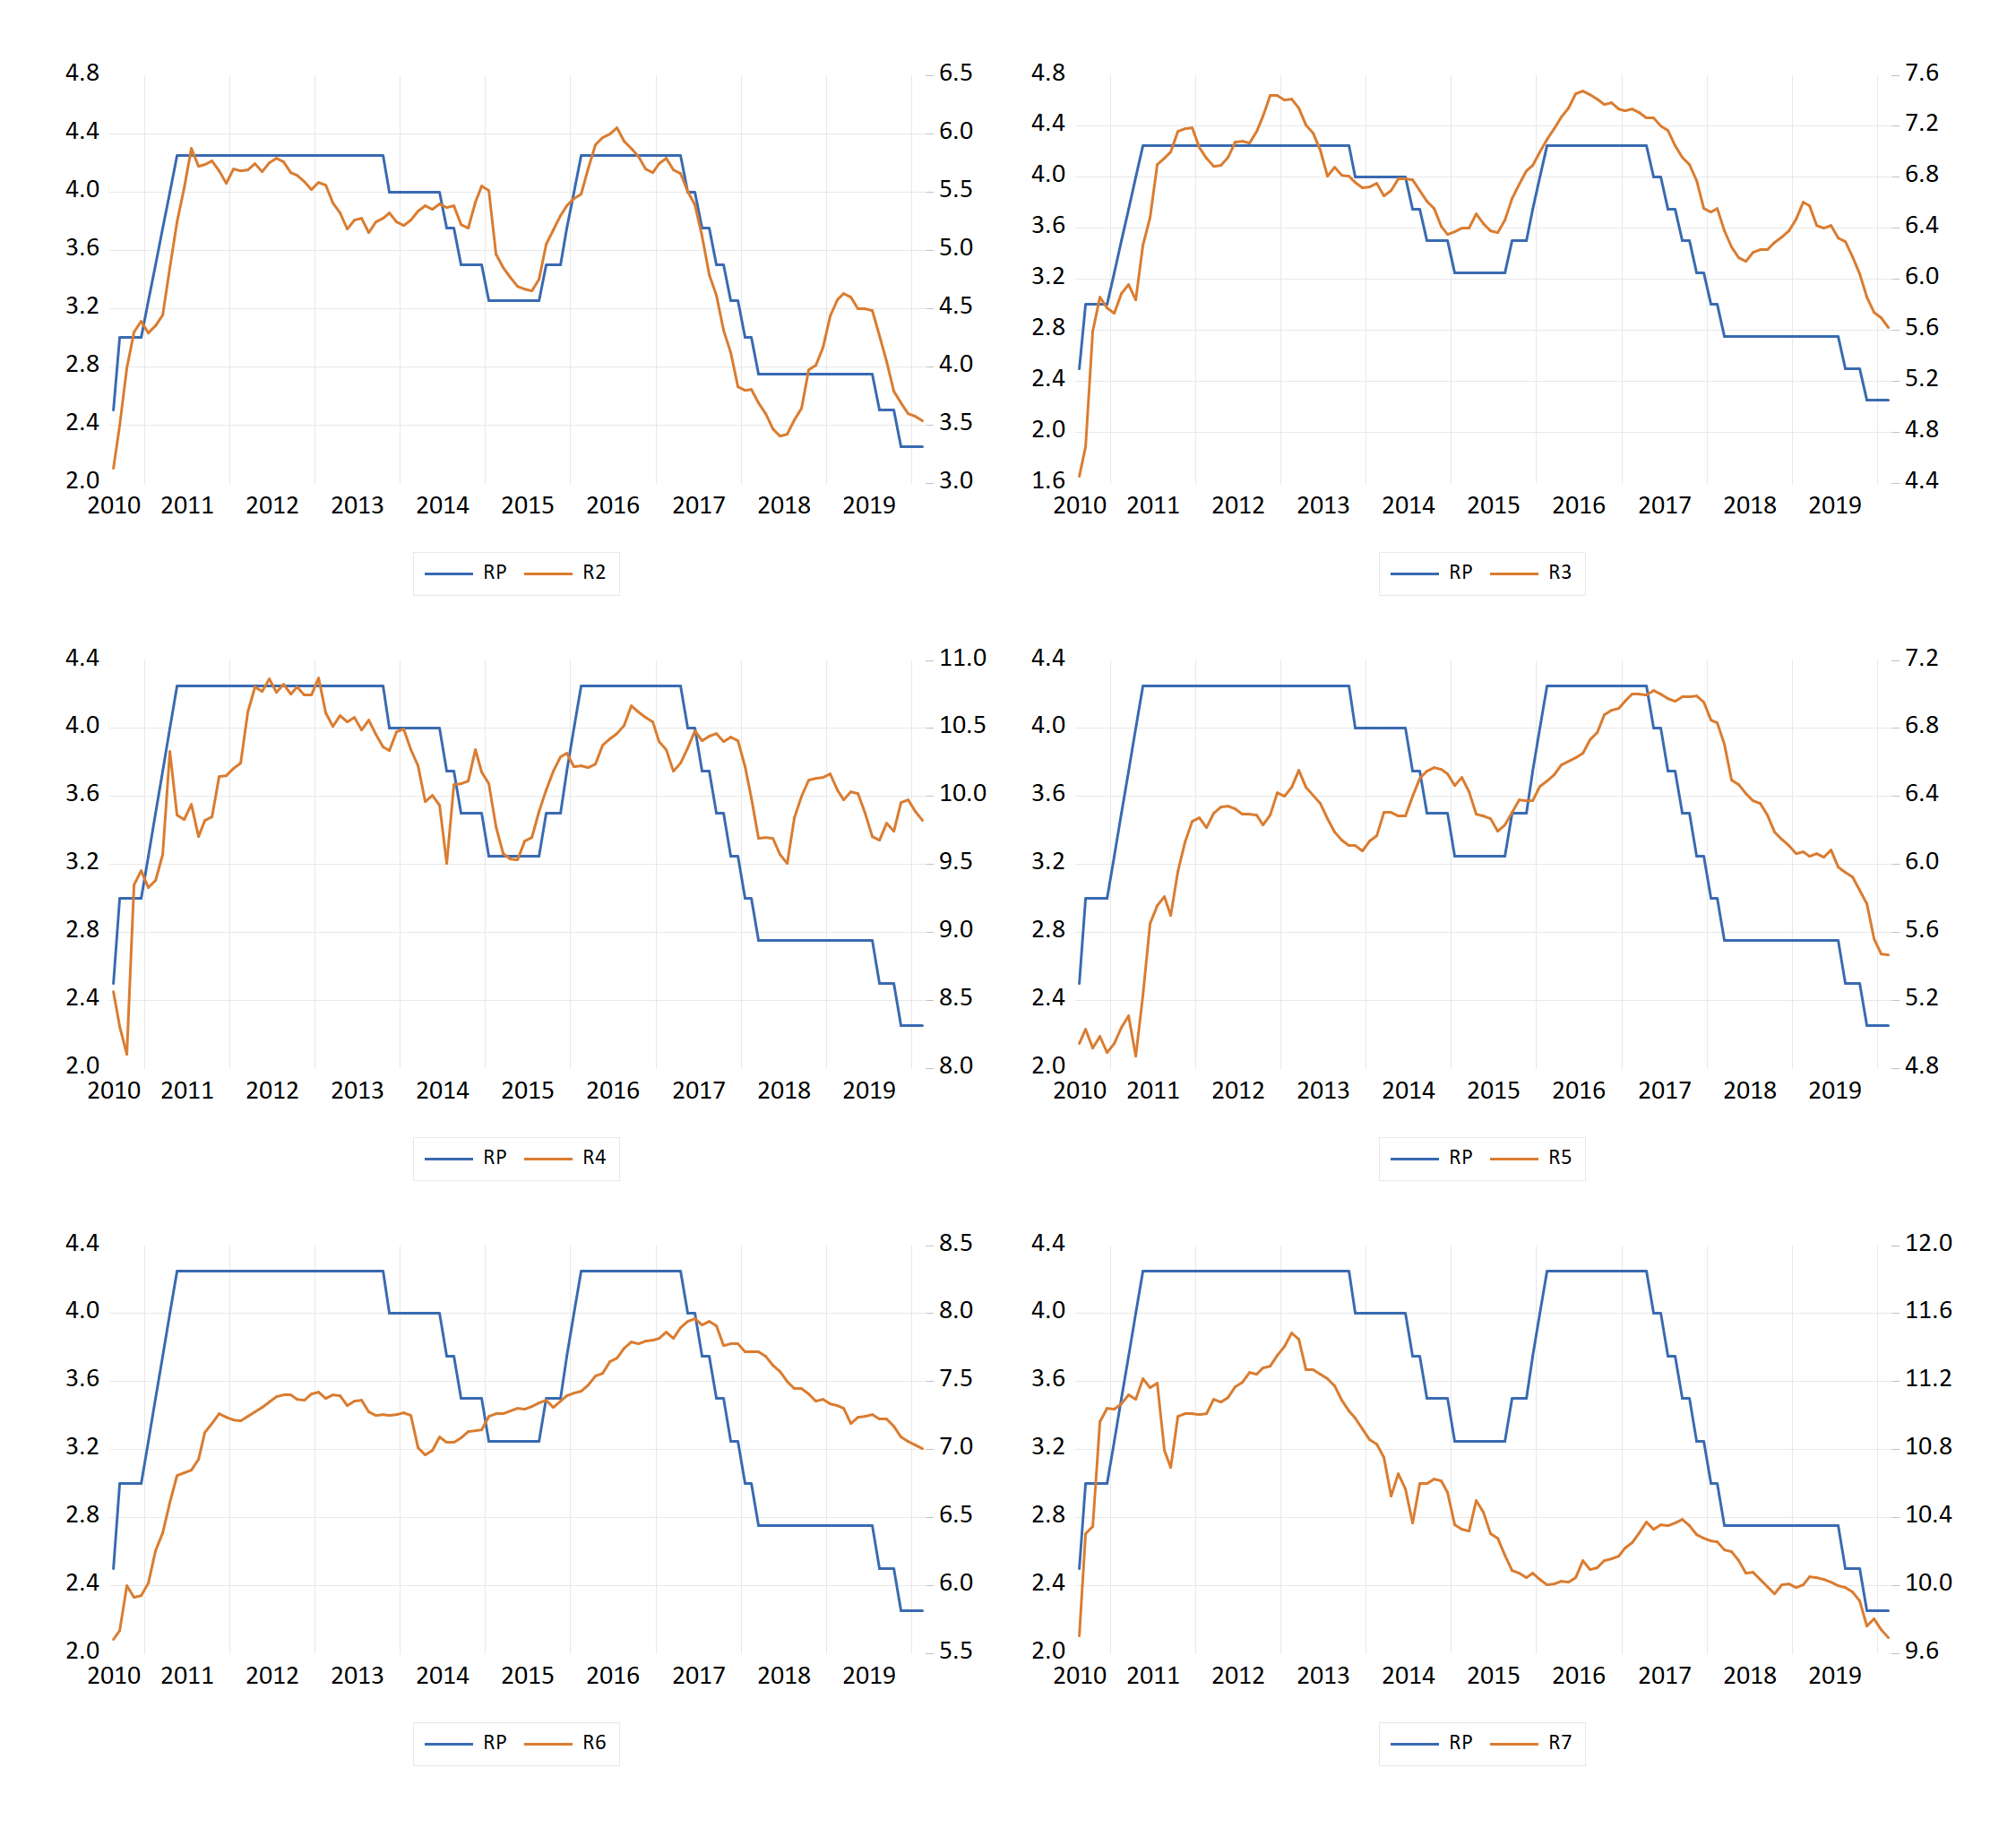
\includegraphics[width=0.95\textwidth]{grafico1_ext_pre.png}
  \caption{Tasa de política monetaria y tasas de préstamos activas de
           corto y largo plazo, submuestra pre-pandemia agosto 2010 --
           febrero 2020.}
  \label{fig:g1pre}
\end{figure}

\begin{figure}[H]
  \centering
  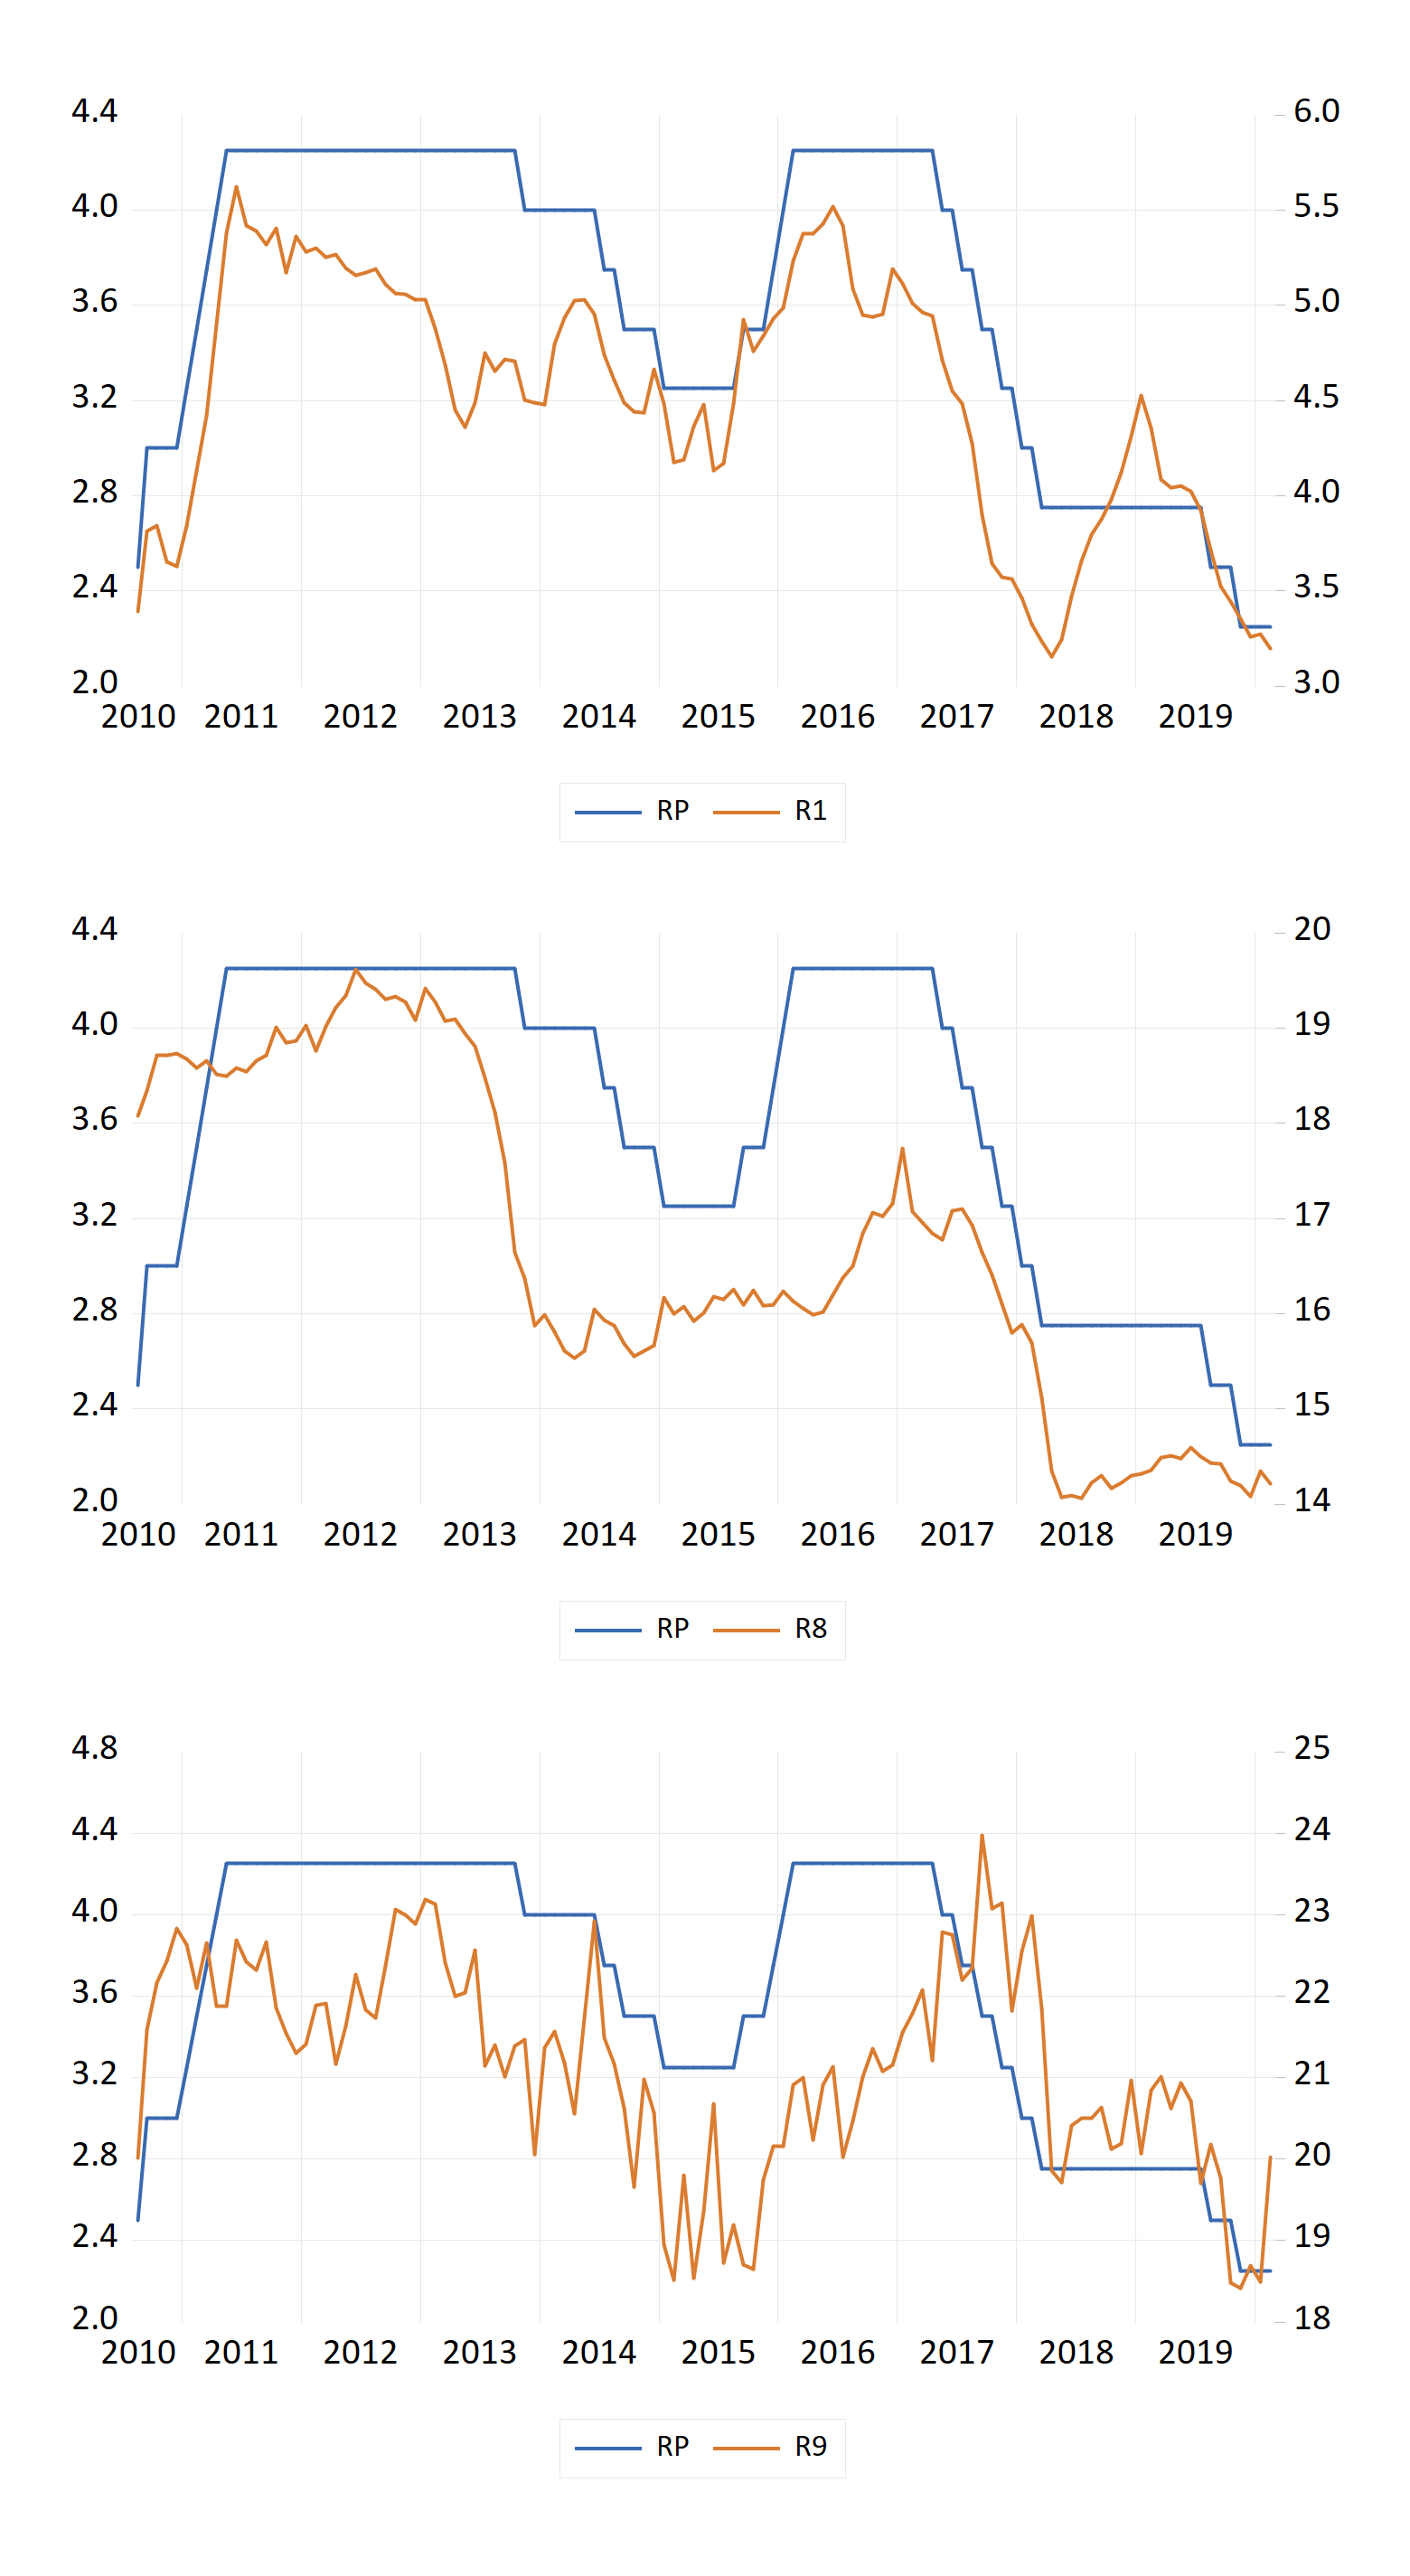
\includegraphics[width=0.95\textwidth]{grafico2_ext_pre.png}
  \caption{Tasa de política monetaria y tasas Preferencial a 90 días,
           TAMN y FTAMN, submuestra pre-pandemia agosto 2010 -- febrero
           2020.}
  \label{fig:g2pre}
\end{figure}

\begin{table}[ht]
\renewcommand{\thetable}{11}
\begin{threeparttable}
\caption{Correlación entre cada tasa activa y la tasa de política
         monetaria, submuestra pre-pandemia 2010--2020}
\label{tab:corrpre}
\small
\begin{tabular}{lcc}
\toprule
Tasa activa & $r$ & prob \\
\midrule
Preferencial 90d         & 0.879 & 0.000 \\
Corporativa $\le$360d    & 0.899 & 0.000 \\
Grandes Emp.\ $\le$360d  & 0.771 & 0.000 \\
Medianas Emp.\ $\le$360d & 0.591 & $3.7\times10^{-12}$ \\
Corporativa $>$360d      & 0.320 & $4.9\times10^{-4}$ \\
Grandes Emp.\ $>$360d    & 0.233 & 0.012 \\
Medianas Emp.\ $>$360d   & 0.642 & $1.1\times10^{-14}$ \\
TAMN                     & 0.709 & 0.000 \\
FTAMN                    & 0.496 & $1.8\times10^{-8}$ \\
\bottomrule
\end{tabular}
\begin{tablenotes}[flushleft]
\footnotesize\item
Frente al Cuadro~8 (muestra completa), TAMN y FTAMN cambian de forma
notable: TAMN sube de $r=0.37$ a $r=0.71$, FTAMN baja de $r=0.79$ a
$r=0.50$. Consistente con que la muestra completa arrastra el ciclo de
subidas sincronizadas de 2021--2023, que infla la correlación lineal
simple de TAMN y FTAMN de maneras distintas entre sí.
\end{tablenotes}
\end{threeparttable}
\end{table}

\begin{table}[ht]
\renewcommand{\thetable}{12}
\caption{Número de rezagos del VAR (criterio de Schwarz), submuestra
         pre-pandemia 2010--2020}
\label{tab:rezagospre}
\centering
\small
\begin{tabular}{lccccccccc}
\toprule
Tasa & R1 & R2 & R3 & R4 & R5 & R6 & R7 & R8 & R9 \\
\midrule
Rezagos & 3 & 3 & 3 & 4 & 1 & 4 & 4 & 3 & 3 \\
\bottomrule
\end{tabular}
\end{table}

\begin{table}[ht]
\renewcommand{\thetable}{13}
\begin{threeparttable}
\caption{Test de traza de Johansen, $H_0{:}\,r=0$, Casos 2 y 3,
         submuestra pre-pandemia 2010--2020}
\label{tab:trazapre}
\small
\begin{tabular}{lcccc}
\toprule
& \multicolumn{2}{c}{Caso 3 (principal)} & \multicolumn{2}{c}{Caso 2 (robustez)} \\
\cmidrule(lr){2-3}\cmidrule(lr){4-5}
Tasa activa & Traza & prob & Traza & prob \\
\midrule
Preferencial 90d         & 14.49 & 0.070 & 14.80 & 0.238 \\
Corporativa $\le$360d    & 12.48 & 0.135 & 12.75 & 0.384 \\
Grandes Emp.\ $\le$360d  & 7.98  & 0.467 & 8.23  & 0.805 \\
Medianas Emp.\ $\le$360d & 15.17 & 0.056 & 15.94 & 0.177 \\
Corporativa $>$360d      & 32.48 & 0.0001 & 33.07 & 0.0005 \\
Grandes Emp.\ $>$360d    & 21.74 & 0.0050 & 23.93 & 0.0149 \\
Medianas Emp.\ $>$360d   & 8.85  & 0.379 & 11.10 & 0.533 \\
TAMN                     & 10.61 & 0.236 & 12.13 & 0.437 \\
FTAMN                    & 6.98  & 0.580 & 7.38  & 0.872 \\
\bottomrule
\end{tabular}
\begin{tablenotes}[flushleft]
\footnotesize\item
Con solo 114 observaciones (frente a 191 en la muestra completa) el
test pierde potencia con claridad: R2, R3, R7, R8 y R9 dejan de
rechazar $H_0$ al 5\,\% bajo ambos casos, cuando algunas sí lo hacían
en la muestra completa (Cuadro~10). Solo R5 y R6 rechazan
consistentemente en las dos muestras y los dos casos.
\end{tablenotes}
\end{threeparttable}
\end{table}

\begin{table}[ht]
\renewcommand{\thetable}{14}
\begin{threeparttable}
\caption{Efecto traspaso y velocidad de ajuste, submuestra
         pre-pandemia 2010--2020 (enfoque uniecuacional, Cuadro 4 pre)}
\label{tab:cuadro4pre}
\small
\begin{tabular}{lccccl}
\toprule
Tasa activa & $\beta_1$ (FMOLS) & $\alpha$ (MCE) & $\theta_0$ (MCE) & Promedio (meses) & Observación\\
\midrule
Preferencial 90d         & 0.86\rlap{***} & $-0.15$\rlap{***} & 0.76\rlap{***} & 0.8  & \\
Corporativa $\le$360d    & 1.06\rlap{***} & $-0.14$\rlap{***} & 0.33\rlap{***} & 5.1  & \\
Grandes Emp.\ $\le$360d  & 0.67\rlap{***} & $-0.20$\rlap{***} & 0.10           & 4.3  & \\
Medianas Emp.\ $\le$360d & 0.45\rlap{***} & $-0.23$\rlap{***} & 0.10           & 3.3  & \\
Corporativa $>$360d      & 0.30\rlap{***} & $-0.05$\rlap{***} & 0.03           & 17.0 & \\
Grandes Emp.\ $>$360d    & 0.18\rlap{*}   & $-0.07$\rlap{***} & 0.09           & 7.0  & \\
Medianas Emp.\ $>$360d   & 0.49\rlap{***} & $-0.03$           & 0.16\rlap{*}   & 21.8 & $\alpha$ no significativo \\
TAMN                     & 1.93\rlap{***} & $-0.02$           & 0.17           & 37.7 & $\alpha$ no significativo \\
FTAMN                    & 0.96\rlap{***} & $-0.22$\rlap{***} & 0.01           & 4.5  & \\
\bottomrule
\end{tabular}
\begin{tablenotes}[flushleft]
\footnotesize
\item * $p<0.10$; ** $p<0.05$; *** $p<0.01$. Números confirmados en
EViews real (Cuadro 4, submuestra pre-pandemia).
\end{tablenotes}
\end{threeparttable}
\end{table}

\begin{table}[ht]
\renewcommand{\thetable}{15}
\begin{threeparttable}
\caption{VAR cointegrado (Johansen), Casos 2 y 3, submuestra
         pre-pandemia 2010--2020 (Cuadro 5 pre)}
\label{tab:cuadro5pre}
\small
\begin{tabular}{lcccc}
\toprule
& \multicolumn{2}{c}{Caso 3 (principal)} & \multicolumn{2}{c}{Caso 2 (robustez)} \\
\cmidrule(lr){2-3}\cmidrule(lr){4-5}
Tasa activa & $\beta_1$ & $\alpha$ & $\beta_1$ & $\alpha$ \\
\midrule
Preferencial 90d         & 0.689 & $-0.132$ & 0.691 & $-0.132$ \\
Corporativa $\le$360d    & 0.922 & $-0.099$ & 0.924 & $-0.098$ \\
Grandes Emp.\ $\le$360d  & 0.728 & $-0.075$ & 0.728 & $-0.075$ \\
Medianas Emp.\ $\le$360d & 0.358 & $-0.194$ & 0.359 & $-0.195$ \\
Corporativa $>$360d      & 0.684 & $-0.065$ & 0.682 & $-0.065$ \\
Grandes Emp.\ $>$360d    & \textbf{0.139} & $-0.057$ & \textbf{0.156} & $-0.059$ \\
Medianas Emp.\ $>$360d   & \textbf{1.035} & $-0.029$ & \textbf{1.019} & $-0.033$ \\
TAMN                     & 2.397 & $-0.034$ & 2.375 & $-0.036$ \\
FTAMN                    & 1.415 & $-0.145$ & 1.385 & $-0.145$ \\
\bottomrule
\end{tabular}
\begin{tablenotes}[flushleft]
\footnotesize\item
Este es, para nosotros, el resultado más importante que aporta esta
submuestra: comparado con el Cuadro 5 extendido de la muestra
completa (arriba), donde R6 daba $\beta_1=-3.55$ (Caso 2, Sección de
robustez con VECM restringido) y R7 daba $\beta_1=-6.66$ -- ambos con
signo económicamente absurdo --, aquí, en la submuestra pre-pandemia,
\textbf{las dos series recuperan un $\beta_1$ de signo correcto y
magnitud razonable} (R6$=0.14$--$0.16$, en línea con su $\beta_1=0.33$
del Cuadro 4 uniecuacional; R7$=1.02$--$1.04$, muy cerca del traspaso
casi completo que reporta el paper original para tasas de corto
plazo). Esto es evidencia adicional a la ya presentada en la
Sección~2.4, de que el problema de R6 y R7 en el VECM de la muestra
completa no es un defecto del método sino algo que introducen
específicamente la pandemia y el ciclo de alzas 2021--2023 en la
identificación de la relación de cointegración de esas dos series.
\end{tablenotes}
\end{threeparttable}
\end{table}

\begin{table}[ht]
\renewcommand{\thetable}{16}
\caption{Efecto traspaso $\beta_1$ (enfoque uniecuacional): paper
         original vs.\ muestra completa vs.\ submuestra pre-pandemia}
\label{tab:comparatres}
\centering
\small
\begin{tabular}{lccc}
\toprule
Tasa activa & Paper (2010--2017) & Completa (2010--2026) & Pre-pandemia (2010--2020) \\
\midrule
Preferencial 90d         & 0.89 & 1.04 & 0.86 \\
Corporativa $\le$360d    & 0.91 & 0.89 & 1.06 \\
Grandes Emp.\ $\le$360d  & 0.98 & 0.81 & 0.66 \\
Medianas Emp.\ $\le$360d & 0.91 & 0.67 & 0.45 \\
Corporativa $>$360d      & 0.39 & 0.27 & 0.30 \\
Grandes Emp.\ $>$360d    & 0.57 & 0.33 & 0.18 \\
Medianas Emp.\ $>$360d   & 0.36 & 0.54 & 0.48 \\
TAMN                     & 1.44 & 0.50 & 1.93 \\
FTAMN                    & 1.33 & 2.16 & 0.96 \\
\bottomrule
\end{tabular}
\end{table}

De esta comparación de tres muestras rescatamos tres lecturas. Primero,
el traspaso de las tasas de corto plazo (R1--R4) se mantiene entre 0.45
y 1.06 en las tres muestras, siempre el más alto del grupo -- el
hallazgo central de \textcite{lahura2017} no depende de si se incluye o
no la pandemia. Segundo, el traspaso de las tasas de largo plazo
(R5--R7) cae de forma bastante consistente del paper (0.36--0.57) a la
pre-pandemia (0.18--0.48) y a la completa (0.27--0.54), lo que sugiere
que refleja un peso creciente de primas de riesgo de plazo cada vez
menos ligadas a la política monetaria de corto plazo. Tercero, TAMN y
FTAMN son,
sin comparación, las series más sensibles a la ventana muestral
elegida (TAMN: 1.44 $\to$ 0.50 $\to$ 1.93; FTAMN: 1.33 $\to$ 2.16
$\to$ 0.96) -- razonable, dado que ambas son promedios móviles de toda
la banca que mezclan una composición de crédito que cambia en el
tiempo.

%%-------------------------------------------------------------
\subsection{Estabilidad estructural del traspaso: hallazgo central
            de la extensión}
%%-------------------------------------------------------------

Dado que la muestra extendida cruza la pandemia y el ciclo de alza de
tasas 2021--2023, sometimos la relación de traspaso a una prueba de
quiebre estructural. La primera versión de esta prueba (Quandt-Andrews
directo sobre la regresión de niveles $R_{i,t}=\beta_0+\beta_1 RP_t+u_t$)
resultó \textbf{metodológicamente inválida}: $R_i$ y $RP$ son ambas
I(1) (Cuadro 2), por lo que esa regresión es cointegrante, no
estacionaria, y la teoría asintótica de \textcite{andrews1993}
para el estadístico sup-$F$ asume regresores I(0) -- aplicarla
directamente sobre una regresión cointegrante puede sobre-rechazar
la hipótesis nula de estabilidad (la teoría correcta para ese caso es
\textcite{hansen1992}, con una distribución asintótica distinta).

La corrección: en vez de probar estabilidad en la ecuación de niveles,
la probamos en la \textbf{ecuación de corto plazo del MCE}, donde los
regresores ($\Delta RP_t$ contemporáneo y el término de corrección de
errores rezagado, estacionario por construcción si existe
cointegración) sí son I(0) y la teoría clásica de Andrews (1993) aplica
sin distorsión. Se testeó quiebre en $\alpha$ (velocidad de ajuste),
en $\theta_0$ (efecto contemporáneo) y conjunto, con recorte simétrico
del 15\,\% en los extremos de la muestra.

\begin{table}[ht]
\renewcommand{\thetable}{7}
\begin{threeparttable}
\caption{Prueba de estabilidad estructural (Quandt-Andrews sobre la
         ecuación de corto plazo del MCE)}
\label{tab:estabilidad}
\small
\begin{tabular}{lccc}
\toprule
Tasa activa & $F$ conjunto ($\alpha,\theta_0$) & $F$ solo $\alpha$ & $F$ solo $\theta_0$ \\
\midrule
Preferencial 90d         & 10.96\rlap{*} & 4.24          & 24.57\rlap{*} \\
Corporativa $\le$360d    & 11.42\rlap{*} & 26.71\rlap{*} & 31.86\rlap{*} \\
Grandes Emp.\ $\le$360d  & 10.46\rlap{*} & 20.30\rlap{*} & 21.00\rlap{*} \\
Medianas Emp.\ $\le$360d &  5.40         &  3.67         & 11.32\rlap{*} \\
Corporativa $>$360d      & 10.80\rlap{*} & 30.64\rlap{*} &  8.86\rlap{*} \\
Grandes Emp.\ $>$360d    &  3.91         &  8.61\rlap{*} &  2.10         \\
Medianas Emp.\ $>$360d   &  6.36         & 14.11\rlap{*} &  4.62         \\
TAMN                     &  4.84         & 11.63\rlap{*} &  1.46         \\
FTAMN                    &  6.37         &  9.01\rlap{*} &  9.43\rlap{*} \\
\bottomrule
\end{tabular}
\begin{tablenotes}[flushleft]
\footnotesize\item
* Significativo al 10\,\%. Valores críticos aproximados (recorte
15\,\%, \textcite{andrews1993}/\textcite{andrewsploberger1994}):
4.87/5.94/8.53 (1 restricción) y 6.42/7.63/10.42 (3 restricciones) a
10/5/1\,\%. Esta descomposición ($F$ conjunto/solo $\alpha$/solo
$\theta_0$) es un cálculo propio en Python, porque EViews no ofrece
una vista que decomponga el sup-$F$ de esta manera. Como confirmación
complementaria (más gruesa, sin la descomposición), sí se corrió en
EViews real la prueba de Quandt-Andrews estándar (\emph{View
$\to$ Stability Diagnostics $\to$ Quandt-Andrews Breakpoint Test})
sobre la ecuación de corto plazo de cada serie: para Medianas Empresas
$>$360d (R7) encontró su máximo estadístico LR-$F$ en 2024m03,
consistente con la inestabilidad ya señalada aquí para esa serie (ver
``Caso especial R7'' más abajo).
\end{tablenotes}
\end{threeparttable}
\end{table}

El hallazgo sobrevive a la corrección metodológica: 6 de 9 series
rechazan estabilidad de parámetros incluso con la versión válida del
test. El patrón por tipo de quiebre es informativo por sí mismo --
Preferencial 90d rompe solo en $\theta_0$ (cambió el efecto
contemporáneo, no la velocidad de ajuste); Corporativa y Grandes
Empresas de corto plazo, Corporativa de largo plazo y FTAMN rompen en
ambos parámetros; Grandes Empresas y Medianas Empresas de largo plazo
y TAMN rompen específicamente en $\alpha$. Medianas Empresas de corto
plazo es la única serie donde la versión corregida del test ya no
rechaza estabilidad al 10\,\% (la versión ingenua sobre niveles sí
rechazaba) -- evidencia concreta de que la corrección metodológica no
fue un ejercicio cosmético.

\textbf{El caso de Grandes Empresas $>$360 días (R6).} Para entender
por qué el Cuadro 5 extendido no produce un resultado interpretable
para esta serie, dividimos la muestra en la fecha de quiebre estimada
sobre la regresión de niveles (abril de 2022) y reestimamos FMOLS por
separado en cada mitad: el efecto traspaso es $\beta_1=1.04$
(EE$=0.09$) antes de abril de 2022, y $\beta_1=-0.68$ (EE$=0.06$)
después -- el signo se invierte. El quiebre en R6 no es solo en la
dinámica de corto plazo: es en el propio \textbf{vector de
cointegración}. El VAR cointegrado de muestra completa está forzando
una única relación de largo plazo sobre dos regímenes genuinamente
distintos, y por eso el algoritmo de máxima verosimilitud no converge
a un resultado con sentido económico -- no es un error de esta
réplica, es el diagnóstico correcto de aplicarle a R6 un modelo que
no debería aplicársele sin permitir el quiebre. Una hipótesis
económica tentativa (no verificada con información adicional): R6 es
la categoría de crédito corporativo de mayor plazo y, presumiblemente,
menor volumen de operaciones, el tipo de serie más expuesta a que el
ciclo de alza 2021--2023 contrajera la demanda de crédito largo de
forma no proporcional al alza de la tasa de política.

\textbf{El caso de Medianas Empresas $>$360 días (R7).} La corrida
real del VECM en EViews reveló, sin haberlo anticipado la verificación
en Python, que R7 exhibe exactamente el mismo patrón ``roto'' que R6:
$\beta_1=-6.66$ y $\alpha=+0.0057$ en el Bloque~1 sin restricciones
(signo económicamente absurdo, raíz explosiva en vez de correctora).
Investigamos esta serie con el mismo tratamiento que R6, con una
complicación adicional: a diferencia de R6, para R7 la prueba de
Quandt-Andrews sobre la ecuación de corto plazo (corrida en EViews
real) y el sup-$F$ sobre la regresión de niveles (calculado en Python,
por consistencia metodológica con el tratamiento de R6) señalan
\textbf{fechas de quiebre distintas} -- 2024m03 la primera, 2020m06 la
segunda. Como verificación de que esta discrepancia es real y no un
error de la implementación propia del sup-$F$, la misma prueba
aplicada a R6 recupera el quiebre de abril de 2022 ya reportado
arriba, lo que confirma que el procedimiento está bien implementado.

Reestimamos FMOLS por separado en las dos mitades de la muestra, para
cada una de las dos fechas candidatas: con el quiebre de 2020m06,
$\beta_1=0.47$ (EE$=0.09$) antes y $\beta_1=0.64$ (EE$=0.13$) después;
con el de 2024m03, $\beta_1=0.57$ (EE$=0.16$) antes y $\beta_1=0.34$
(EE$=0.17$) después (el FMOLS de muestra completa, sin partir, da
$\beta_1=0.57$, EE$=0.14$). En \textbf{ninguna} de las cuatro
sub-muestras el coeficiente cambia de signo -- se mantiene en un rango
moderado y económicamente sensato (0.34 a 0.64) -- a diferencia de R6,
donde el mismo ejercicio (FMOLS pre/post) sí produce una inversión de
signo real (de 1.04 a $-0.68$). Como verificación adicional, calculamos
también el FMOLS de muestra completa para R6: da $\beta_1=0.35$
(EE$=0.11$), un valor moderado y sensato, muy distinto del
$\beta_1=-3.55$ que arroja su VECM de muestra completa -- el mismo
patrón (FMOLS estable, VECM explosivo) se repite en R6 y en R7.

La lectura más defendible, con esta evidencia, es que el patrón
``roto'' de R7 refleja sobre todo una \textbf{fragilidad del método de
estimación de sistema completo (VECM/Johansen)}, no necesariamente un
quiebre real en la relación de cointegración de largo plazo entre R7 y
$RP$: R7 ya cointegraba solo al margen del 10\,\% por Engle-Granger
($p=0.054$, Cuadro 3), y el estimador de sistema completo es
conocidamente más sensible que el uniecuacional (Engle-Granger/FMOLS)
cuando la cointegración de partida ya es marginal. Esto contrasta con
R6, donde el propio FMOLS -- no solo el VECM -- muestra una inversión
de signo real al partir la muestra, evidencia de que ahí sí hay un
quiebre genuino en el vector de cointegración.

Como evidencia complementaria -- y más intuitiva que una tabla de
estadísticos $F$ -- estimamos el efecto traspaso en ventanas móviles
de 72 meses (Gráfico~3). El código completo está en el Anexo~A.10; la
primera versión de este gráfico tenía un error de especificación
(extraía la constante de cada FMOLS rodante en vez de la pendiente
$\beta_1$, documentado como ``Corrección 6'' en el Anexo~A.10) que
produjo valores sin sentido económico (varias series entre 3 y 19);
el gráfico de abajo ya está corregido y confirmado en EViews real.

\begin{figure}[ht]
  \centering
  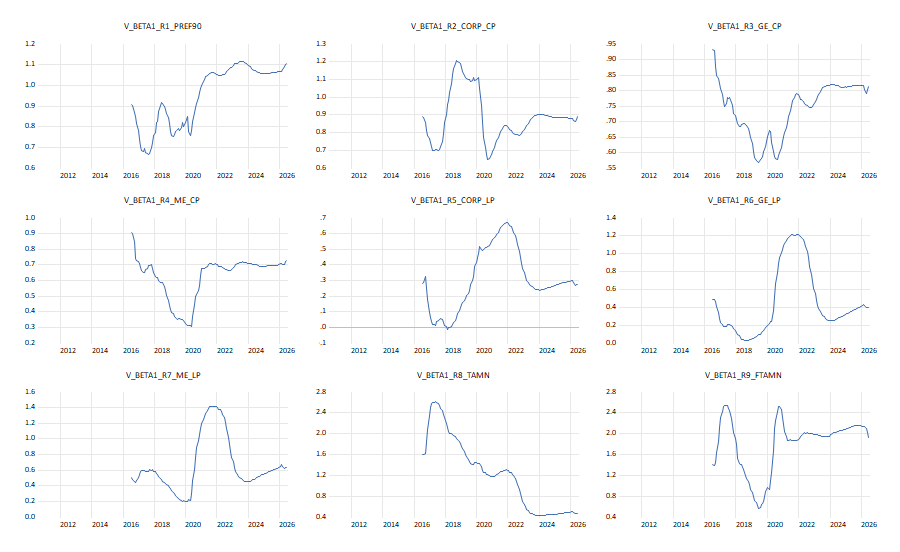
\includegraphics[width=0.95\textwidth]{grafico_rolling.png}
  \caption{Efecto traspaso ($\beta_1$) en ventanas móviles de 72 meses,
           FMOLS, una por cada una de las 9 tasas activas.}
  \label{fig:rolling}
\end{figure}

El patrón más llamativo del Gráfico~3 es que la mayoría de las series
muestra un quiebre visible alrededor de 2018--2022 -- coincidiendo con
la pandemia y el inicio del ciclo de alza de tasas --, no solo las que
ya señalamos como problemáticas en el Cuadro 5. TAMN (R8) y FTAMN (R9)
suben con fuerza hasta 2016--2018, caen hacia 2020, y después TAMN
sigue descendiendo hasta ubicarse cerca de 0.3--0.5 hacia 2026,
mientras FTAMN rebota a un rango de 2.0--2.8. Grandes Empresas y
Medianas Empresas de largo plazo (R6 y R7) muestran una dinámica muy
parecida entre sí: ambas caen a un mínimo cercano a 0.1--0.2 alrededor
de 2018--2020 y luego repuntan abruptamente a un pico de 1.2--1.6 hacia
2020--2022, antes de normalizarse de nuevo en 0.4--0.6 -- coherente con
la inestabilidad de ambas series ya documentada arriba. Corporativa de
largo plazo (R5) es la única serie que llega a cruzar por debajo de
cero (mínimo apenas negativo) alrededor de 2018--2020, la evidencia
más visual de que es la serie con el traspaso más frágil de las 9.

\textbf{Conclusión de esta sección.} La muestra extendida no debería
tratarse como una única relación estable de traspaso para las 9
series por igual. R6 y R7 son los dos casos donde el VECM de muestra
completa deja de ser interpretable, pero por razones que no son
idénticas: en R6 la propia relación de cointegración (el FMOLS
uniecuacional) cambia de signo al partir la muestra, evidencia de un
quiebre genuino; en R7 el FMOLS se mantiene razonablemente estable en
todas las sub-muestras, y el diagnóstico más plausible es que sea el
método de estimación de sistema completo el que se vuelve frágil
cuando la cointegración de partida ya es marginal, más que un cambio
real en la relación de largo plazo. Un tratamiento riguroso y completo
de esta extensión requeriría, como mínimo, permitir un quiebre
estructural endógeno en la relación de cointegración misma para R6 (y,
en menor medida, contrastar formalmente la hipótesis de fragilidad del
método frente a la de quiebre genuino para R7 y R8) --
metodologías como \textcite{gregoryhansen1996} (que extiende
Engle-Granger a un quiebre endógeno en la regresión de cointegración)
o la extensión de Johansen con quiebre de \textcite{johansenmosconinielsen2000}
son la vía natural. Dado el alcance de esta pregunta (4 puntos) y el
tiempo disponible antes de la entrega, documentamos aquí el
diagnóstico completo -- con evidencia formal de que es real y no un
artefacto de una prueba mal aplicada -- en vez de implementar esas dos
metodologías adicionales, que quedan identificadas como la extensión
natural de este trabajo.

Vale la pena notar que este diagnóstico no depende únicamente de
nuestro ejercicio de sub-muestras (Gráfico 3, arriba): el análisis de
robustez pre-pandemia de la Sección~2.3, con una partición de muestra
distinta, apunta exactamente en la misma dirección -- R6 y R7 son las
únicas dos series cuyo VECM de muestra completa deja de tener sentido
económico y que, al recortar la muestra justo antes de la pandemia,
recuperan un $\beta_1$ de signo correcto (Cuadro~15). Que dos
ejercicios distintos, con particiones de muestra distintas, coincidan
en señalar a las mismas dos series es, para nosotros, la evidencia más
convincente de todo este trabajo de que el problema es real y no un
artefacto de cómo se cortó la muestra en un ejercicio en particular.

\clearpage
%%=============================================================
\section*{Anexo}
\addcontentsline{toc}{section}{Anexo}
%%=============================================================

Este anexo documenta, tal como exige el enunciado del examen, (A) el
código EViews completo empleado, (B) los procedimientos que se
ejecutaron manualmente en la interfaz gráfica de EViews porque no
tienen equivalente por línea de comandos, y (C) la metodología de
verificación cruzada con Python empleada para encontrar las
especificaciones parsimoniosas que replican los Cuadros 4 y 5.

\textbf{Estructura del proyecto.} Todo el material del examen (código,
datos, documento y paper original) está organizado en una única
carpeta de proyecto, \texttt{ef\_pucp/}, con la siguiente estructura:

\begin{verbatim}
ef_pucp/
|-- template/
|   |-- content.tex          documento principal (este archivo)
|   |-- content.pdf          documento compilado
|   |-- referencias.bib      bibliografia BibLaTeX / APA 7
|   `-- figures/
|       |-- grafico1.png / grafico2.png                 Graficos 1-2 (Pregunta 1)
|       |-- grafico1_ext.png / grafico2_ext.png         Graficos 1-2 extendidos (muestra completa)
|       |-- grafico1_ext_pre.png / grafico2_ext_pre.png Graficos 1-2 (submuestra pre-pandemia)
|       `-- grafico_rolling.png                          traspaso rodante (Seccion 2.4)
|-- codes/                   12 archivos .prg de EViews (Anexo A)
|   |-- P1_1a_correlaciones_graficos.prg
|   |-- P1_1b_paneles_finales.prg
|   |-- P1_2a_cuadro2_raizunitaria.prg
|   |-- P1_2b_cuadro3_englegranger.prg
|   |-- P1_2c_cuadro3_resumen.prg
|   |-- P1_3a_cuadro4_mce_lineal.prg
|   |-- P1_3b_cuadro4_resumen.prg
|   |-- P1_3c_cuadro4_mce_no_lineal.prg
|   |-- P1_4a_cuadro5_var_johansen.prg
|   |-- P1_4b_cuadro5_resumen.prg
|   |-- P1_4c_cuadro5_mce_no_lineal.prg
|   `-- P2_1_extension_completa.prg      Pregunta 2 completa (Anexo A.10)
|-- data/
|   |-- bcrp_series.ipynb                  script de descarga P1 (Anexo C.1)
|   |-- bcrp_series_p2.py                  script de descarga P2, muestra extendida
|   |-- tasas_interes_lahura2017.xlsx/.csv panel P1 (82 obs., ago.2010-may.2017)
|   |-- tasas_interes_lahura2017_ext.xlsx/.csv panel P2 (191 obs., ago.2010-jun.2026)
|   |-- tasas_interes_lahura2017.wf1       workfile EViews
|   `-- BCRPData-metadata-*.csv            catalogo de series BCRP
|-- ef_metriamacro.pdf        enunciado del examen final
|-- nota_semanal/             [solo local, no en GitHub] 5 Notas Semanales BCRP (verificacion TAMN, Anexo C)
|-- referencias_pdf/          [solo local, no en GitHub] PDFs con copyright
|-- .gitignore
`-- README.md                 guia completa del proyecto y su estado
\end{verbatim}

Los archivos \texttt{.prg} de \texttt{codes/} se referencian desde este
documento vía \lstinline{\lstinputlisting} (Anexo~A), por lo que deben
mantenerse como carpeta hermana de \texttt{template/} para que el
documento compile (ver Anexo~A). El repositorio completo, con
historial de versiones de cada script y del propio documento, está
disponible en GitHub:
\url{https://github.com/alejandroventuraventurameza-tech/lahura_2017_replication}.
Ahí también
se encuentra el \texttt{README.md} con el detalle completo del estado
de la réplica -- qué valores son exactos, cuáles son aproximados y
cuáles no se lograron reproducir, con la investigación documentada
detrás de cada caso -- pensado para que cualquier lector externo pueda
seguir el trabajo sin depender de este documento. La carpeta
\texttt{referencias\_pdf/} (el paper de Lahura y los tres artículos
metodológicos citados en el Anexo C.6) y el PDF del enunciado del
examen se excluyen del repositorio (\texttt{.gitignore}) por tratarse
de material con derechos de autor de terceros; se conservan solo en la
copia local del proyecto.

%%-------------------------------------------------------------
\subsection*{A. Código EViews}
\addcontentsline{toc}{subsection}{A. Código EViews}
%%-------------------------------------------------------------

Todos los archivos siguen la convención de nombres
\texttt{P1\_<pregunta><parte>\_<contenido>.prg} y se ejecutan en el
orden en que aparecen (cada uno indica su prerrequisito en el
encabezado de comentarios).

\subsubsection*{A.1. Gráficos 1 y 2 -- construcción de correlaciones y
                    paneles (\texttt{P1\_1a})}
\lstinputlisting[language=EViews]{../codes/P1_1a_correlaciones_graficos.prg}

\subsubsection*{A.2. Gráficos 1 y 2 -- paneles finales
                    (\texttt{P1\_1b})}
\lstinputlisting[language=EViews]{../codes/P1_1b_paneles_finales.prg}

\subsubsection*{A.3. Cuadro 2 -- pruebas de raíz unitaria
                    (\texttt{P1\_2a})}
\lstinputlisting[language=EViews]{../codes/P1_2a_cuadro2_raizunitaria.prg}

\subsubsection*{A.4. Cuadro 3 -- cointegración Engle-Granger
                    (\texttt{P1\_2b})}
\lstinputlisting[language=EViews]{../codes/P1_2b_cuadro3_englegranger.prg}

\subsubsection*{A.4b. Cuadro 3 -- tabla resumen (\texttt{P1\_2c})}
\lstinputlisting[language=EViews]{../codes/P1_2c_cuadro3_resumen.prg}

\subsubsection*{A.5. Cuadro 4 -- MCE lineal, enfoque uniecuacional
                    (\texttt{P1\_3a})}
\lstinputlisting[language=EViews]{../codes/P1_3a_cuadro4_mce_lineal.prg}

\subsubsection*{A.5b. Cuadro 4 -- tabla resumen (\texttt{P1\_3b})}
\lstinputlisting[language=EViews]{../codes/P1_3b_cuadro4_resumen.prg}

\subsubsection*{A.6. Cuadro 4 -- MCE no lineal, extra crédito
                    (\texttt{P1\_3c})}
\lstinputlisting[language=EViews]{../codes/P1_3c_cuadro4_mce_no_lineal.prg}

\subsubsection*{A.7. Cuadro 5 -- VAR cointegrado / Johansen, enfoque
                    multiecuacional (\texttt{P1\_4a})}
\lstinputlisting[language=EViews]{../codes/P1_4a_cuadro5_var_johansen.prg}

\subsubsection*{A.8. Cuadro 5 -- tabla resumen (\texttt{P1\_4b})}
\lstinputlisting[language=EViews]{../codes/P1_4b_cuadro5_resumen.prg}

\subsubsection*{A.9. Cuadro 5 -- MCE no lineal, extra crédito
                    (\texttt{P1\_4c})}
\lstinputlisting[language=EViews]{../codes/P1_4c_cuadro5_mce_no_lineal.prg}

\subsubsection*{A.10. Pregunta 2 completa -- Gráficos 1--2, Cuadros
                    2--5 extendidos y extensión de estabilidad
                    estructural (\texttt{P2\_1\_extension\_completa})}
\lstinputlisting[language=EViews]{../codes/P2_1_extension_completa.prg}

%%-------------------------------------------------------------
\subsection*{B. Procedimientos manuales (no automatizables por
              línea de comandos)}
\addcontentsline{toc}{subsection}{B. Procedimientos manuales}
%%-------------------------------------------------------------

EViews 12 no expone algunos pasos de la interfaz gráfica a través de la
ventana de comandos. Estos procedimientos se documentan aquí como
flujogramas en pseudocódigo, en el orden y con el nombre exacto de cada
opción de menú, para que sean reproducibles por cualquier lector con
acceso a EViews.

\textbf{B.1. Prueba de cointegración de Johansen (Cuadro 3).}
La vista \textit{Group / Cointegration Test / Johansen System
Cointegration Test...} siempre abre un diálogo interactivo, incluso
pasando argumentos por comando (\lstinline{group.coint(2,1,N)} prellena
el rezago pero igual requiere confirmación manual). Procedimiento
seguido para cada una de las 9 tasas activas:
\begin{enumerate}
  \item Abrir el grupo \texttt{gg\_<serie>} (contiene \texttt{RP\_REF}
        y la tasa activa correspondiente, creado en \texttt{P1\_1a}).
  \item \textit{View} $\to$ \textit{Cointegration Test} $\to$
        \textit{Johansen System Cointegration Test...}
  \item En el diálogo: \textit{Deterministic trend assumption} $\to$
        seleccionar opción \textbf{"2) Intercept (no trend) in CE - no
        intercept in VAR"}.
  \item \textit{Lag intervals for D(endogenous)}: dejar el rezago
        prellenado \texttt{1 N}, donde \texttt{N} es el rezago que
        reporta el Cuadro 3 del paper para esa serie en la columna
        Johansen.
  \item \textit{Critical values}: verificar que esté marcada
        \textbf{MacKinnon-Haug-Michelis (1999)} (opción por defecto).
  \item \textit{OK}. Copiar la tabla de resultado (\textit{Trace test},
        filas \textit{None} y \textit{At most 1}) -- probabilidad de
        $H_0{:}\,r=0$ y $H_0{:}\,r=1$, respectivamente.
  \item Repetir para las 9 series y transcribir los 18 valores a la
        tabla \texttt{CUADRO\_3} (\texttt{P1\_2c}).
\end{enumerate}

\textbf{B.2. Corrección del supuesto de tendencia por defecto en
objetos VAR/VEC (Cuadro 5).} El comando
\lstinline{var <nombre>.ec(1) <lag_lo> <lag_hi> <lista>} crea el
objeto VAR/VEC sin abrir diálogo, pero SIEMPRE con el supuesto de
tendencia por defecto (Caso 3: ``Intercept (no trend) in CE and VAR''),
distinto del Caso 2 que exige la nota del Cuadro 5. No existe forma de
pasar el caso de tendencia como argumento del comando
(\lstinline{.ec(1,2)} y \lstinline{.ec(1,rc)} arrojan error). Se
corrige a mano, para \textbf{cada} objeto VAR nuevo:
\begin{enumerate}
  \item Doble clic en el objeto \texttt{V\_<serie>} para abrirlo.
  \item \textit{Estimate} $\to$ pestaña \textit{Cointegration}.
  \item Seleccionar el radio-botón \textbf{"2) Intercept (no trend)
        in CE - no intercept in VAR"} (por defecto viene marcada la
        opción 3).
  \item \textit{OK}. (Este ajuste no se hereda entre objetos: hay que
        repetirlo cada vez que se crea un VAR/VEC nuevo.)
\end{enumerate}

\textbf{B.3. Restricciones sobre el vector de cointegración y la
matriz de ajuste (Bloques 2--4 del Cuadro 5).} Sobre el mismo objeto
\texttt{V\_<serie>} ya con el Caso 2 aplicado:
\begin{enumerate}
  \item \textit{Estimate} $\to$ pestaña \textit{VEC Restrictions}.
  \item Escribir las restricciones en la caja de texto, una por línea,
        con la sintaxis nativa de EViews. Ejemplo (traspaso completo):
        \lstinline{B(1,1)=1} seguido de \lstinline{B(1,2)=-1}.
        Ejemplo (traspaso incompleto + exogeneidad débil, serie con
        $\beta_1$ ya identificado, p.ej.\ R2): \lstinline{B(1,1)=1},
        \lstinline{B(1,2)=-0.750}, \lstinline{A(2,1)=0}.
  \item En \textit{Optimization control}: \textit{Max Iterations}
        $=500$ (se amplió del valor por defecto para confirmar
        convergencia); \textit{Convergence} $=0.0001$ (por defecto).
  \item \textit{OK}. EViews reporta automáticamente el \textit{LR test
        for binding restrictions} (estadístico $\chi^2$ y
        probabilidad) que se transcribe a los bloques 2--4 del
        Cuadro 5.
\end{enumerate}

\textbf{B.4. Eje dual en los Gráficos 1 y 2.} No se encontró sintaxis
de línea de comandos para asignar una serie a un eje secundario dentro
de un objeto \textit{Graph}. Para cada uno de los 9 paneles:
\begin{enumerate}
  \item Doble clic sobre la línea de la tasa de mercado (color naranja
        por defecto, la segunda serie del grupo).
  \item \textit{Graph Options} $\to$ \textit{Series axis assignment}.
  \item En la fila correspondiente a esa serie, marcar \textbf{Right}.
  \item \textit{Apply} $\to$ \textit{OK}.
\end{enumerate}

%%-------------------------------------------------------------
\subsection*{C. Conexión con Python: metodología de búsqueda y
              verificación cruzada}
\addcontentsline{toc}{subsection}{C. Conexión con Python}
%%-------------------------------------------------------------

El paper no publica el algoritmo exacto de poda ``general-a-específico''
usado para llegar a los MCE parsimoniosos de los Cuadros 4 y 5, ni la
fórmula exacta del Promedio en el caso no lineal. Para las series donde
la poda manual en EViews no reproducía a la primera los valores
publicados, se usó Python como banco de pruebas rápido antes de
confirmar la especificación ganadora en EViews real -- nunca al revés
(Python nunca reemplaza la verificación en EViews, solo acota el
espacio de búsqueda).

\textbf{C.1. Descarga de datos.} Las 9 series de tasas activas y la
tasa de referencia se descargaron con un script Python
(\texttt{bcrp\_series.ipynb}, en \texttt{ef\_pucp/data/}) que consulta,
serie por serie, el endpoint público de BCRPData
\url{https://estadisticas.bcrp.gob.pe/estadisticas/series/api/<código>/json/<inicio>/<fin>}
(nunca varias series en una sola URL, para evitar un error de orden
documentado de esa API), verificando cada código contra el catálogo
oficial de metadatos del BCRP (\texttt{BCRPData-metadata-*.csv}) y
contra el API en vivo, para la muestra \texttt{2010-8} a \texttt{2017-5}
(agosto 2010 -- mayo 2017, 82 observaciones mensuales sin datos
faltantes, igual que \textcite{lahura2017}). Los 10 códigos de serie
exactos usados en la réplica de la Sección~1 son:

\begin{center}
\small
\begin{tabular}{llc}
\toprule
Variable & Descripción & Código BCRP \\
\midrule
$R_1$   & Preferencial corporativa a 90 días      & \texttt{PN07809NM} \\
$R_2$   & Corporativa $\le$360 días                & \texttt{PN07801NM} \\
$R_3$   & Grandes Empresas $\le$360 días            & \texttt{PN07802NM} \\
$R_4$   & Medianas Empresas $\le$360 días           & \texttt{PN07803NM} \\
$R_5$   & Corporativa $>$360 días                   & \texttt{PN07804NM} \\
$R_6$   & Grandes Empresas $>$360 días               & \texttt{PN07805NM} \\
$R_7$   & Medianas Empresas $>$360 días              & \texttt{PN07806NM} \\
$R_8$   & TAMN                                        & \texttt{PN07807NM} \\
$R_9$   & FTAMN                                       & \texttt{PN07808NM} \\
$R_P$   & Tasa de referencia de política monetaria   & \texttt{PD04722MM} \\
\bottomrule
\end{tabular}
\end{center}

El panel resultante se exporta a \texttt{.xlsx}/\texttt{.csv}
(\texttt{tasas\_interes\_lahura2017.xlsx/.csv}, en
\texttt{ef\_pucp/data/}) con la fecha en el formato que reconoce el
asistente de importación de EViews (\texttt{2010m08}, \ldots). El
mismo notebook descarga además, para uso futuro y no usado en esta
réplica, las 8 tasas pasivas $R_{10}$--$R_{17}$ y la tasa interbancaria
del Cuadro 1 del paper (19 series en total).

\textbf{C.2. Búsqueda combinatoria de especificaciones parsimoniosas.}
Para cada serie problemática se construyó, en \texttt{numpy}/
\texttt{pandas}, la matriz de diseño con hasta 16 rezagos candidatos
(8 de $\Delta R_i$ y 8 de $\Delta RP$) y se evaluaron por mínimos
cuadrados todas las combinaciones de 0 a 5--6 rezagos extra (cientos a
decenas de miles de modelos por serie), comparando el $\alpha$ y
$\theta_0$ resultantes contra los valores redondeados publicados. Este
método identificó, entre otras, la especificación exacta de R8 (Cuadro
4) y las 5 series con asimetría del Cuadro 4 no lineal.

\textbf{C.3. Estimación conjunta (SUR) para el Cuadro 5.} Un hallazgo
central del trabajo (ver Sección~1.3) es que estimar la ecuación
$\Delta R_{i,t}$ del bloque restringido del Cuadro 5 por MCO
uniecuacional, ignorando su correlación con la ecuación
$\Delta RP_t$, da un resultado \textbf{distinto} al de la estimación
conjunta que usa EViews internamente para el VAR cointegrado
restringido. Se implementó mínimos cuadrados generalizados factibles
iterado (SUR): dado un vector de coeficientes, se calcula la matriz de
covarianza de residuos $2\times2$ (dividiendo por $n-k_1$, no por
$n$, para reproducir los errores estándar de EViews), se resuelven las
ecuaciones normales apiladas ponderadas por $\hat\Sigma^{-1}$, y se
repite hasta convergencia. Validado contra el output nativo de EViews
para R2 (Corporativa $\le$360d): $\beta_1=0.750$, $\alpha=-0.1993$
(Python) vs.\ $\beta_1=0.750$, $\alpha=-0.1992$ (EViews), diferencia
atribuible solo a redondeo.

\textbf{C.4. Reconstrucción del intercepto exacto de FMOLS.} Para
series ``sin constante'' en el MCE (p.\,ej.\ R8/TAMN), el intercepto
$\beta_0$ de la ecuación de cointegración FMOLS no queda implícito en
la regresión del MCE (a diferencia de las series ``con constante'',
donde cualquier $\beta_0$ es absorbido por el intercepto libre). Se
solicitó al usuario el output completo de \lstinline{eq_fmols_R8_tamn.output}
en EViews para obtener $\beta_0=11.66597$ con precisión completa, en
vez de aproximarlo; con este valor exacto la búsqueda combinatoria
amplia (más de 30,000 especificaciones, incluyendo rezagos hasta orden
14) confirmó que ninguna especificación alternativa reproduce el
Promedio publicado de TAMN (69.2), reforzando la conclusión de que se
trata de una imprecisión de la tabla original y no de una
especificación no encontrada.

\textbf{C.5. Pruebas de imposibilidad matemática.} Para las dos filas
del Cuadro 4 donde el Promedio publicado resultó irreproducible (R5 y
R7), se acotó algebraicamente el rango de valores posibles del
Promedio dado el bracket de redondeo (2 decimales) de $\alpha$,
$\theta_0$ y $\beta_1$ ya confirmados, demostrando que el valor
impreso queda \textbf{fuera} de ese rango en ambos casos --
independientemente de qué combinación de rezagos se use. Esto
distingue una imprecisión de imprenta (R5, R7) de un caso donde la
especificación correcta simplemente no se ha encontrado (R8, donde el
valor publicado sí es matemáticamente alcanzable).

\textbf{C.6. Revisión de las fuentes metodológicas del MCE no lineal
multiecuacional (Cuadro 5, R3/R4).} Lahura (2017) señala en su
introducción que sus MCEs son similares a los de
\textcite{heffernan1997}, \textcite{sander2004} y \textcite{hofmann2004}.
Ante la brecha persistente entre la velocidad de ajuste replicada y la
publicada para R3 y R4 (única fila del Cuadro 5 con asimetría), se
obtuvieron y revisaron a fondo los tres artículos citados en busca del
algoritmo exacto de estimación del sistema con término de corrección
de errores partido. Heffernan (1997) resultó ser un MCE uniecuacional
simétrico con rezagos fijos (sin selección de modelo), sin tratar
asimetría. Hofmann y Mizen (2004) sí modelan asimetría con un término
partido idéntico en espíritu al de Lahura, pero de forma
\textit{siempre} uniecuacional (nunca como sistema de ecuaciones
simultáneas), por lo que informan el enfoque uniecuacional (Cuadro 4,
ya replicado con alta precisión) pero no el multiecuacional. Sander y
Kleimeier (2004) usan la misma convención de umbral en cero
(especificación ``TAR0''), con selección de rezagos por AIC (máximo 4,
simétricos); esta regla exacta se probó en Python y \textbf{empeoró}
el ajuste en vez de mejorarlo. Se probaron además variantes con el
término contemporáneo $\Delta RP_t$ y con la restricción de
exogeneidad débil relajada (esta última confirmó que la restricción
original es la correcta: el coeficiente adicional resultó no
significativo), la precisión del $\beta_1$/intercepto impuestos en el
bloque restringido (validada de forma independiente: reproduce 30/30
valores primarios exactos en las 5 series con Bloque 4, ver Anexo~A.7,
por lo que se descarta como fuente del error), y la inclusión del
régimen $u^{+}_{t-1}$ (no significativo). Tras múltiples vías de
investigación independientes documentadas en \texttt{P1\_4c}, el
$\alpha$ de esta fila no se pudo replicar con la información
metodológica pública disponible -- mismo estándar aplicado a R5/R7/R8
(Cuadro 4) y al Bloque 4 original de R2 (Cuadro 5, ver Anexo~A.7). Sin
embargo, se identificó que el Promedio de Cuadro 5' usa la misma
fórmula de Hendry \parencite{hendry1995} que el MCE lineal (no
$-1/\alpha$, como se documentó inicialmente): el propio Promedio
impreso por el paper para R3 y R4 no es autoconsistente con su propio
$\alpha$ bajo $-1/\alpha$, lo que reveló el error de convención. Con
la fórmula corregida y una especificación con término contemporáneo
confirmada en EViews real, el Promedio reportado mejoró sustancialmente
(Grandes Empresas $\le$360d: de 5.6 a 3.5, objetivo 4.1; Medianas
Empresas $\le$360d: de 2.9 a 1.5, objetivo 1.1), dejando al $\alpha$
como el único valor no exacto de esta fila.

%%=============================================================
%% BIBLIOGRAFÍA
%%=============================================================
\clearpage
\pagestyle{plain}
\printbibliography[title={Referencias}]

\end{document}
